% IMPORTANT: PLEASE USE XeLaTeX FOR TYPESETTING
%!TEX program = pdflatex 
\documentclass[aspectratio=169,10pt]{beamer}
\usetheme{Darmstadt}%{default}

%% PACKAGES POUR BEAMER

\usetheme{metropolis}
\usepackage[utf8]{inputenc}
\usepackage[T1]{fontenc}
\usepackage[french]{babel}
\usepackage{appendixnumberbeamer}
\usepackage{booktabs}
\usepackage[scale=2]{ccicons}
\usepackage{xspace}
\newcommand{\themename}{\textbf{\textsc{metropolis}}\xspace}
%%
\usepackage{bookmark}
\usepackage{tikz}
\usepackage{wrapfig}
\usepackage{multicol}
\usepackage{subfig}
\usepackage{color} % package des couleurs
\usepackage{xcolor}
\usepackage{graphicx}
\usepackage{pgfplots}
\usetikzlibrary{plotmarks}
\usepackage{pst-all}
\usepackage{lmodern}
\usepackage{multimedia}
\usepackage{media9}
\usepackage{cancel}

%% style des pages
\usepackage{fancyhdr}
%\pagestyle{fancy}

\usepackage{multimedia}
\usepackage{media9}
\usepackage[framemethod=tikz]{mdframed}

%% maths
\DeclareMathOperator{\e}{e}
\usepackage{mathtools}
\usepackage{amsfonts}
\usepackage{amsmath}
\usepackage{amssymb}
\usepackage{hyperref}
\usepackage{esvect}
\usepackage{upgreek}
\usetikzlibrary{shadows}
\usetikzlibrary{backgrounds}
\usepackage{transparent}



%% environnements


\definecolor{definitionf}{RGB}{220,252,220}
\definecolor{definitionl}{RGB}{39,123,69}
\definecolor{definitiono}{RGB}{72,148,101}


%%%%%%%%%% DEFINITION
\newmdenv[tikzsetting={fill=definitionf}, linewidth=2pt, linecolor=definitionl, outerlinewidth=0pt, innertopmargin=5pt, innerbottommargin=5pt, innerleftmargin=5pt, innerrightmargin=5pt, leftmargin=0pt]{defi}

\newmdenv[ tikzsetting={drop shadow={ shadow xshift=1ex, shadow yshift=-1em, fill=definitiono, opacity=1, every shadow } }, outerlinewidth=2pt, outerlinecolor=white, linecolor=white, innertopmargin=0pt, innerbottommargin=0pt, innerleftmargin=0pt, innerrightmargin=0pt]{ombredef}



%%%%%%%%%% THEOREME
\definecolor{theof}{RGB}{255,216,218}
\definecolor{theol}{RGB}{160,0,4}
\definecolor{theoo}{RGB}{221,65,100}


\newmdenv[tikzsetting={fill=theof}, linewidth=2pt, linecolor=theol, outerlinewidth=0pt, innertopmargin=5pt, innerbottommargin=5pt, innerleftmargin=5pt, innerrightmargin=5pt, leftmargin=0pt]{theo}

\newmdenv[ tikzsetting={drop shadow={ shadow xshift=1ex, shadow yshift=-0.5em, fill=theoo, opacity=1, every shadow } }, outerlinewidth=2pt, outerlinecolor=white, linecolor=white, innertopmargin=0pt, innerbottommargin=0pt, innerleftmargin=0pt, innerrightmargin=0pt]{ombretheo}

%%%%%%%%%%%%%%%%%%%%%%%%%%%%%%%%%%%%%%%%%%%%%%%%%%%%%%%%%%%%%%%%%%%%%%%%%%%%%%%%
%% Logo

% %% Insert the logo figures here
% \titlegraphic{%
%   \centering
%   %\hspace{3cm}
%   \vspace{-.5cm}
%     
\includegraphics[scale=.2]{figures/logo_univ_paris.png}\hspace{3cm}
%     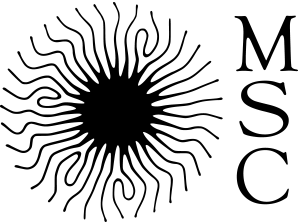
\includegraphics[scale=4]{figures/msc.png}\hspace{2cm}
%     
\includegraphics[scale=.13]{figures/anr-logo.png}\hfill
% }
%%%%%%%%%%%%%%%%%%%%%%%%%%%%%%%%%%%%%%%%%%%%%%%%%%%%%%%%%%%%%%%%%%%%%%%%%%%%%%%%

%%%%%%%%%%%%%%%%%%%%%%%%%%%%%%%%%%%%%%%%%%%%%%%%%%%%%%%%%%%%%%%%%%%%%%%%%%%%%%%%
%% Title page

% \makeatletter
% \setbeamertemplate{title page}{
%   \begin{minipage}[t][\paperheight]{\textwidth}
%     \ifx\inserttitle\@empty\else\usebeamertemplate*{title}\fi
%     \ifx\insertsubtitle\@empty\else\usebeamertemplate*{subtitle}\fi
%     \usebeamertemplate*{title separator}
%     \begin{center}
%     \ifx\beamer@shortauthor\@empty\else\usebeamertemplate*{author}\fi
%     \ifx\insertinstitute\@empty\else\usebeamertemplate*{institute}\fi
%     \ifx\insertdate\@empty\else\usebeamertemplate*{date}\fi
    
%     \end{center}
%     \vspace{.3cm}
%     \ifx\inserttitlegraphic\@empty\else\inserttitlegraphic\fi
%     %\vspace*{.2cm}
%   \end{minipage}
% }

%% FOOTLINE
\setbeamertemplate{footline}{
\leavevmode%

\hbox{\hspace*{-0.06cm}
\begin{beamercolorbox}[wd=.2\paperwidth,ht=2.25ex,dp=1ex,center]{author in head/foot}%
%\usebeamerfont{author in head/foot}\insertshortauthor\hfill
\insertframenumber{} / \inserttotalframenumber\hspace*{2ex}
\end{beamercolorbox}%

\begin{beamercolorbox}[wd=.6\paperwidth,ht=2.25ex,dp=1ex,center]{section in head/foot}%
\usebeamerfont{section in head/foot}%\insertshorttitle
\end{beamercolorbox}%

\begin{beamercolorbox}[wd=.2\paperwidth,ht=2.25ex,dp=1ex,right]{section in head/foot}%
%\usebeamerfont{section in head/foot}\hspace*{2em}
\usebeamerfont{section in head/foot}
%\insertframenumber{} / \inserttotalframenumber\hspace*{2ex}
\end{beamercolorbox}}%

\vskip0pt%
}
\makeatother

%%%%%%%%%%%%%%%%%%%%%%%%%%%%%%%%%%%%%%%%%%%%%%%%%%%%%%%%%%%%%%%%%%%%%%%%%%%%%%%%



\usecolortheme{beaver}
\usefonttheme{serif}
\usepackage{lmodern}
\usepackage{hyperref}
\usepackage{multimedia}
 % pour un pdf lisible à l'écran
 % il y a d'autres choix possibles 
\usepackage{pslatex}
% \usepackage{ctex, hyperref}
\usepackage{latexsym,amsmath,xcolor,multicol,booktabs,calligra}
\usepackage{graphicx,pstricks,listings,stackengine}

\definecolor{cobalt}{rgb}{0.0, 0.28, 0.67}
\usepackage{tcolorbox}
  \tcbuselibrary{most} 
  \tcbset{colback=cobalt!5!white,colframe=cobalt!75!black}

\definecolor{aquamarine}{rgb}{0.5, 1.0, 0.83}
\definecolor{applegreen}{rgb}{0.55, 0.71, 0.0} 
\newtcolorbox{Programme}[1]{
	colback=cobalt!5!white,
  	colframe=cobalt!65!black,
	fonttitle=\bfseries,
  	title={#1}}  


\graphicspath{{figures/}}

% meta-data
\title{Mise en Perspective du Dossier Didactique de Recherche}
\subtitle{Agrégation externe spéciale de Physique Chimie: option Physique}
\author{\large Gabriel Le Doudic}
\date{}
%\institute{Préparation à l'agrégation de Rennes 1}
% \titlebackground{images/background}

% document body
\begin{document}
\maketitle
% --------- Sommaire ---------
% \begin{frame}
%     \tableofcontents
% \end{frame}      
% ----------------------------
% \section{Introduction}

\begin{frame}{Parcours de formation à et par la recherche}
  \centering
\begin{minipage}{.32\linewidth}
\centering

\includegraphics[width=.25\linewidth]{./figures/etudes.jpg}\smallskip

\textbf{CPGE PCSI/PC}\smallskip

Lycée Lapérouse kerichen - Brest - 2012-2015\smallskip

\textbf{Magistère de Physique Fondamentale}\smallskip

Université Paris-Saclay - Orsay - 2015-2018\smallskip

\textbf{Master Dynamique des Fluides et Énergétique (DFE)}\smallskip

Université Paris-Saclay - Orsay - 2018\smallskip


\end{minipage}\hfill
\begin{minipage}{.3\linewidth}
  \centering
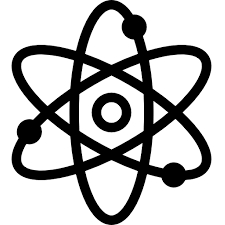
\includegraphics[width=.25\linewidth]{./figures/stages.jpg}\smallskip

\textbf{\textcolor{red}{Stage de Licence 3}}\smallskip

LPS - Université Paris-Saclay - 2 mois \smallskip

\textbf{\textcolor{red}{Stage de Master 1}}\smallskip

MSC - Université Paris-Cité - 3 mois\smallskip

\textbf{\textcolor{red}{Stage de Master 2}}\smallskip

FAST - Université Paris-Saclay - 6 mois 

\vfill
\end{minipage}\hfill
\begin{minipage}{.32\linewidth}
  \centering

\includegraphics[width=.25\linewidth]{./figures/these.jpg}\smallskip


\textbf{\textcolor{blue}{Thèse de physique}}\smallskip

\textbf{\og{}Écoulements solutocapillaires en présence d'échange interface-volume: génération de vorticité interfaciale et propulsion\fg{}}\smallskip

Dirigée par Dr. Mattieu \bsc{ROCHÉ} et Dr. Laurent \bsc{LIMAT}
 soutenue le 31 janvier 2022\smallskip

Laboratoire Matière et Systèmes Complexes
\end{minipage}
\end{frame}

\section{Mes travaux de recherche}

\begin{frame}{I. Écoulements solutocapillaires en présence d'échange interface-volume: génération de vorticité interfaciale et propulsion}
    \begin{figure}[!ht]
        \begin{minipage}[c]{.45\textwidth}
        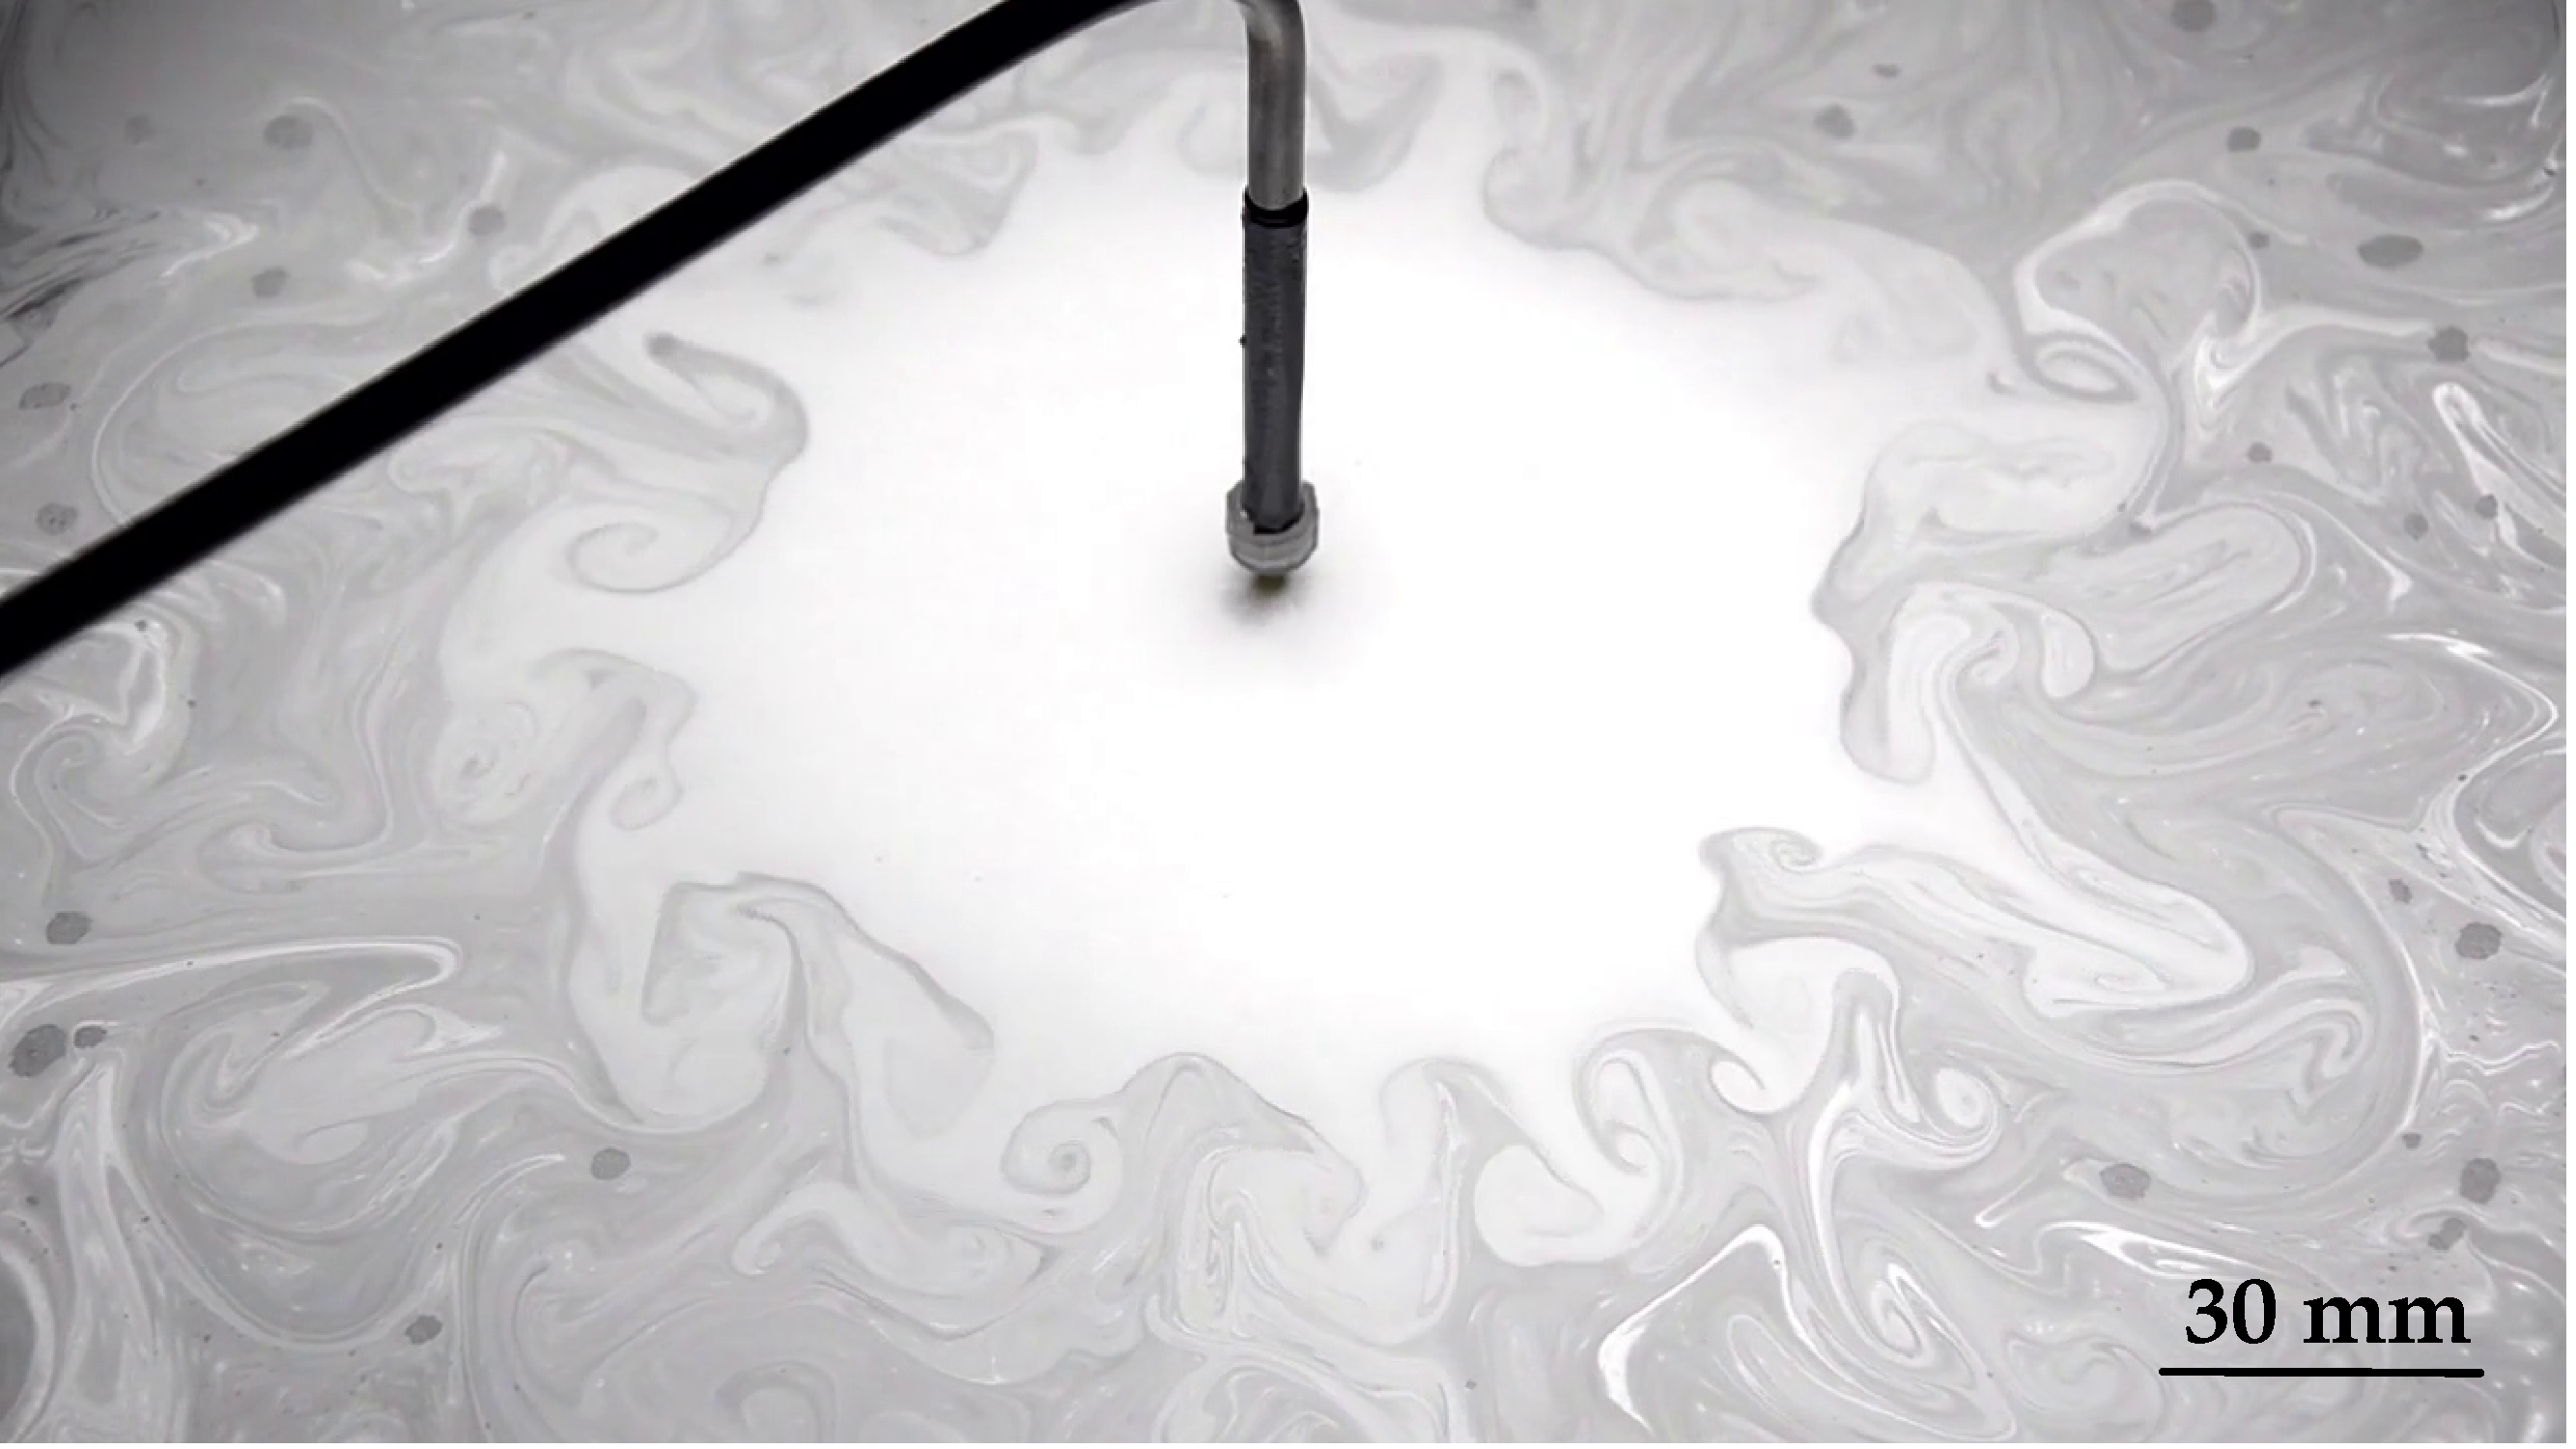
\includegraphics[width=1\textwidth]{./figures/Ecoulement_Marangoni.pdf}
        \captionof{figure}{Écoulement de Marangoni solutal}
        \end{minipage}\hfill
        \begin{minipage}[c]{.45\textwidth}
        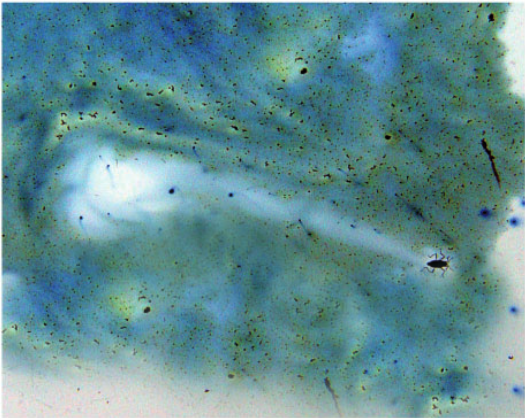
\includegraphics[width=.72\textwidth]{./figures/microvelia.png}
        \captionof{figure}{Propulsion par effet Marangoni, [Andersen $1982$]}
        \end{minipage}
    \end{figure}
\end{frame}

% \begin{frame}{1.1. L'origine de la tension de surface}
%     \begin{figure}
%       \centering
%       \input{./figures/Marangoni_effect_general_1.tex}
%     \end{figure}
% \end{frame}


% \begin{frame}{1.1. L'origine de la tension de surface}
%     \begin{minipage}[c]{5cm}
%     \begin{figure}
%      \centering
%      \resizebox{1\textwidth}{!}{\input{./figures/DefInterface_Gibbs.pdf_tex}}
%    \end{figure}
  
%   \end{minipage}
%   \begin{minipage}[c]{7cm}
%    \textbf{Énergie libre de Gibbs du système:}
%    \begin{eqnarray}
%      dG = VdP-SdT+\sum_{i}\mu_i dN_i+\gamma d\mathcal{A},\\
%      dG_{\rm total} = dG^{\alpha}+dG^{\beta}+dG^{\sigma}\nonumber
%    \end{eqnarray}
  
%    \textbf{à $T,~P,~N_i$ constants:}%
  
%    \begin{equation}
%      \left.\frac{\partial G_{\rm total}}{\partial \mathcal{A}}\right|_{T,V,N^{\alpha, \beta}} = \gamma(N_i, T)
%    \end{equation}
%   \end{minipage}
%   \end{frame}

  % \begin{frame}{1.4. Diminution de la tension de surface par ajout de tensioactifs}
  %   \begin{figure}
  %     \includegraphics[scale=.8]{./figures/tensioactif1.pdf}\footnote{[Bergeron 1997]}
  %   \end{figure}
  % \end{frame}

  \begin{frame}{I.1. La tension de surface}
    \begin{minipage}{6cm}
      \noindent \textbf{$\bullet$ Situation à l'équilibre:}
    \begin{figure}
     \centering
     \resizebox{.9\textwidth}{!}{\input{./figures/DefInterface_Gibbs.pdf_tex}}
   \end{figure}
   \begin{equation}
   \left.\frac{\partial G_{\rm total}}{\partial \mathcal{A}}\right|_{T,P,N^{\alpha, \beta}} = \gamma(N_i, T)
   \end{equation}
    \end{minipage}\hfill
    \begin{minipage}{6cm}
    \textbf{Situation hors équilibre:}
    \begin{ombredef}
      \begin{defi}
    \[\Delta \gamma = \gamma_0-\gamma(c,T)\neq 0\]
    $\Delta\gamma$ induit une contrainte à l'interface
      \end{defi}
    \end{ombredef}

      \begin{figure}
        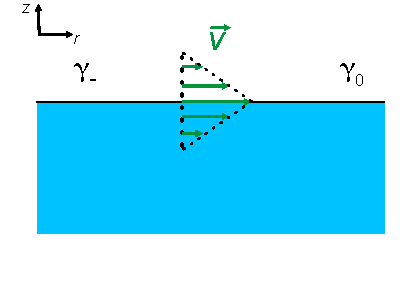
\includegraphics[width=1\textwidth]{./figures/contrainte.pdf}
      \end{figure}
    \end{minipage}
  \end{frame}

  \begin{frame}{I.2. Description hydrodynamique de l'écoulement}
    \noindent \textbf{$\bullet$  Équation de Navier Stokes}
    %\begin{Programme}{Équation de Navier-Stokes:}
      \begin{equation}
        \rho\left(\dfrac{\partial \vec{v}}{\partial t}+\left(\vec{v}\cdot\vec{\rm grad}\right)\vec{v}\right)=-\vec{\rm grad}p+\eta\Delta\vec{v}.\label{eq:NS1}
      \end{equation}
    %\end{Programme}
  \noindent \textbf{$\bullet$ Conservation de la masse:}
    \begin{equation}
    \dfrac{\partial \rho}{\partial t}+\vec{\nabla}\cdot\vec{j}_m(M,t)=0\Rightarrow\vec{\nabla}\cdot \vec{v} = 0
  \end{equation} 

  \noindent \textbf{$\bullet$ Équation de convection-diffusion du tensioactif en volume et à la surface}
    \begin{equation}
      \begin{array}{ccc}      
  \dfrac{\partial c}{\partial t}+\left(\vec{c}\cdot \vec{\nabla}\right)c = D\Delta c & \text{et} &  \dfrac{\partial \Gamma}{\partial t}+\dfrac{1}{r}\frac{\partial }{\partial r}\left(rv_r\Gamma\right) = -D\Delta c 
      \end{array}
\end{equation}
  \noindent\textbf{$\bullet$  Conditions aux limites à la surface du liquide} %\begin{Programme}{Conditions aux limites à la surface du liquide}
    \begin{figure}
      \centering
      \begin{tikzpicture}
        \draw (0,0) node{$
        \text{En}~z=0~ \eta\left(\frac{\partial v_r}{\partial z}+\frac{\partial v_z}{\partial r}\right) = \frac{\partial \gamma}{\partial r},\text{   avec   } \gamma(r)=\gamma_0-\|\dfrac{\partial \gamma}{\partial c}\|c(r,0).$};
        \draw [red, very thick] (-0.3,0) circle (.35);
        \draw [red, very thick] (0,-0.2) -- (0.3,-.5) node[right]{Moteur de l'écoulement};
      \end{tikzpicture}
    \end{figure}

  \end{frame}

  % \begin{frame}{I.3.  Conditions aux limites}
  %   \textbf{$\bullet$ Conditions aux limites à la surface du liquide:}
  %   \begin{figure}
  %     \centering
  %     \begin{tikzpicture}
  %       \draw (0,0) node{\large $
  %       \eta\left(\frac{\partial v_r}{\partial z}+\frac{\partial v_z}{\partial r}\right) = \frac{\partial \gamma}{\partial r}, ~\text{en}~z=0.$};
  %       \draw [red, very thick] (0.45,0) circle (.35);
  %       \draw [red, very thick] (0.6,-.3) -- (0.9,-.5) node[right]{Moteur de l'écoulement};
  %     \end{tikzpicture}
  %   \end{figure}
  %     \textbf{$\bullet$ Écoulement solutocapillaire}
  %     \begin{itemize}
  %       \item équation de convection-diffusion du tensioactif;
  %       $$ \frac{\partial \Gamma}{\partial t}+\frac{1}{r}\frac{\partial }{\partial r}\left(rv_r\Gamma\right) = -D\Delta c$$
  %       \item variation de $\gamma$ avec la concentration:
  %       $$\frac{\partial\gamma}{\partial r}=\frac{\gamma_0-\gamma(c)}{R}$$
  %     \end{itemize}
  % \end{frame}

  \begin{frame}{I.3. Dépôt d'une goutte de tensioactif}
    \begin{minipage}{.4\textwidth}
    %\begin{figure}
      \centering
      \resizebox{!}{.8\textwidth}{%% : Introduction à l'effet Marangoni

\begin{tikzpicture}[scale=1]
  \shade [top color = white, bottom color=cyan] (-5,0) -- (5,0) -- (5,3) -- (-5,3) -- cycle;
  \shade [top color = blue!60, bottom color = white] (-5,0) -- (5,0) -- (5,-3) -- (-5,-3) -- cycle;
  \draw[very thick] (-5,0) -- (5,0);

  \draw (-4,.5) node{Fluide n$^{\circ}1$};
  \draw (4,-.5) node{Fluide n$^{\circ}2$};
  \draw (4,.5) node{$\boldsymbol{\gamma}\textbf{+}$};
  \draw (-4,-.5) node{$\boldsymbol{\gamma}\textbf{+}$};
  \foreach \x in {-1,-.5,-.2, 0, .2, .5, 1} \draw[fill=black] (\x,-.1) circle (.1);
  
           %\foreach \x in {1,2,3} {$x=\x$, }
  \foreach \x in {-1,-.5,-.2,0,.2,.5,1} \draw[black] (\x,0)--(\x,.3) ;
  
  \draw (0,.8) node{$\boldsymbol{\gamma}\textbf{-}$};
  \draw (0,-.7) node{Tensioactif};
  
  \draw [latex-latex](-3,-2)--(3,-2) node[below, midway]{ $\frac{\Delta c}{R} \Rightarrow \frac{\Delta \gamma}{R} \Rightarrow v_{\rm surfacique}$};
 
\end{tikzpicture}
}
      %\end{figure}
    \end{minipage}\hfill
    \begin{minipage}{.5\textwidth}
      \centering
      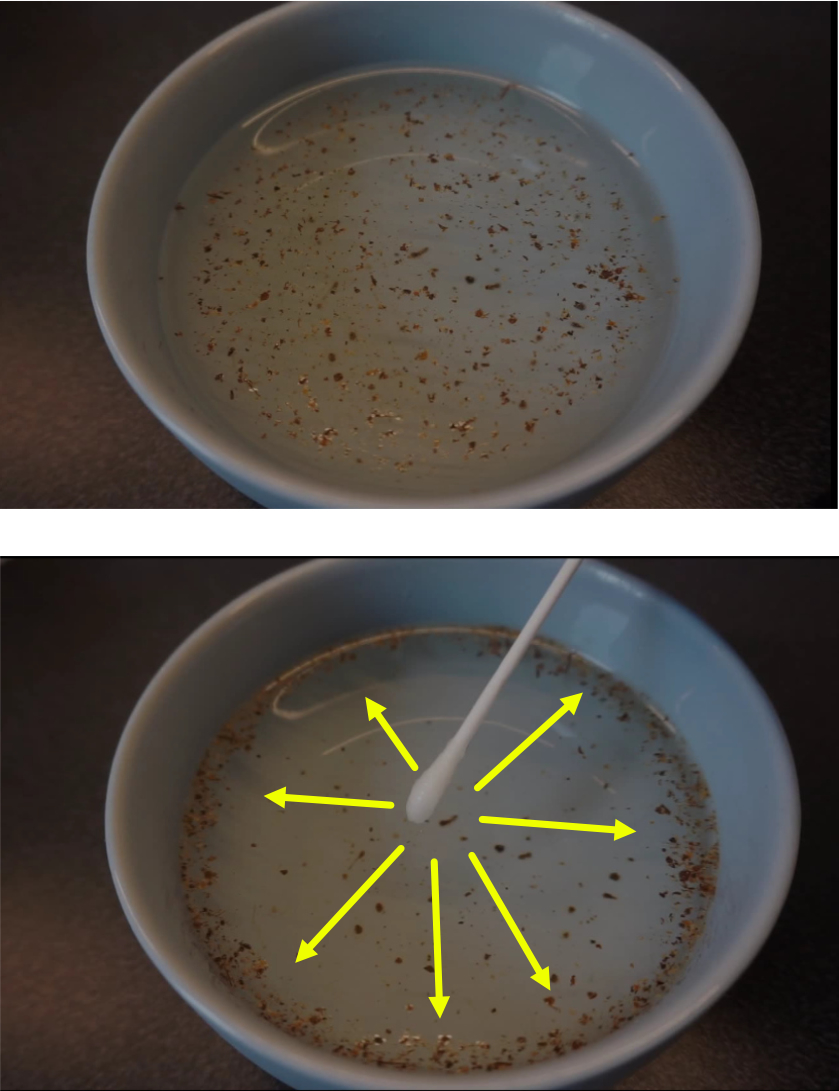
\includegraphics[width=.6\textwidth]{./figures/Distanciation_v3.jpg}
    \end{minipage}
  \end{frame}

  % \begin{frame}{I.3. Dépôt d'une goutte de tensioactif}
  %   \begin{figure}
  %     \movie{\resizebox{1\textwidth}{!}{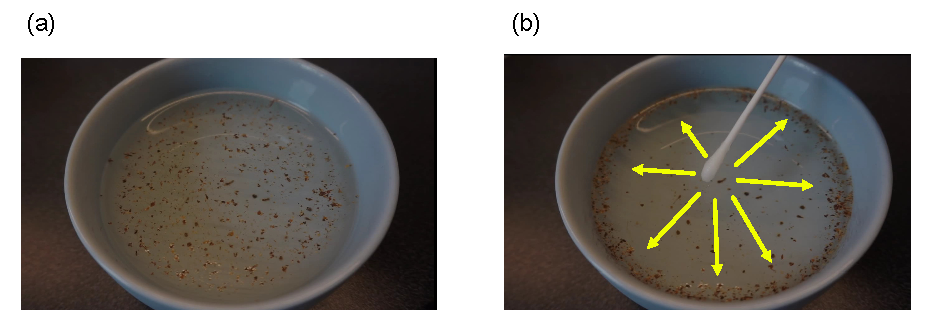
\includegraphics[width=1\textwidth]{./figures/Distanciation_v2.pdf}}}{./videos/Marangoni_poivre.avi}
    
  %   \end{figure}
  %   \end{frame}
    

    \begin{frame}{I.4. Écoulement de Marangoni à flux constant}
      \begin{minipage}{.45\textwidth}
        \begin{figure}
          \centering
          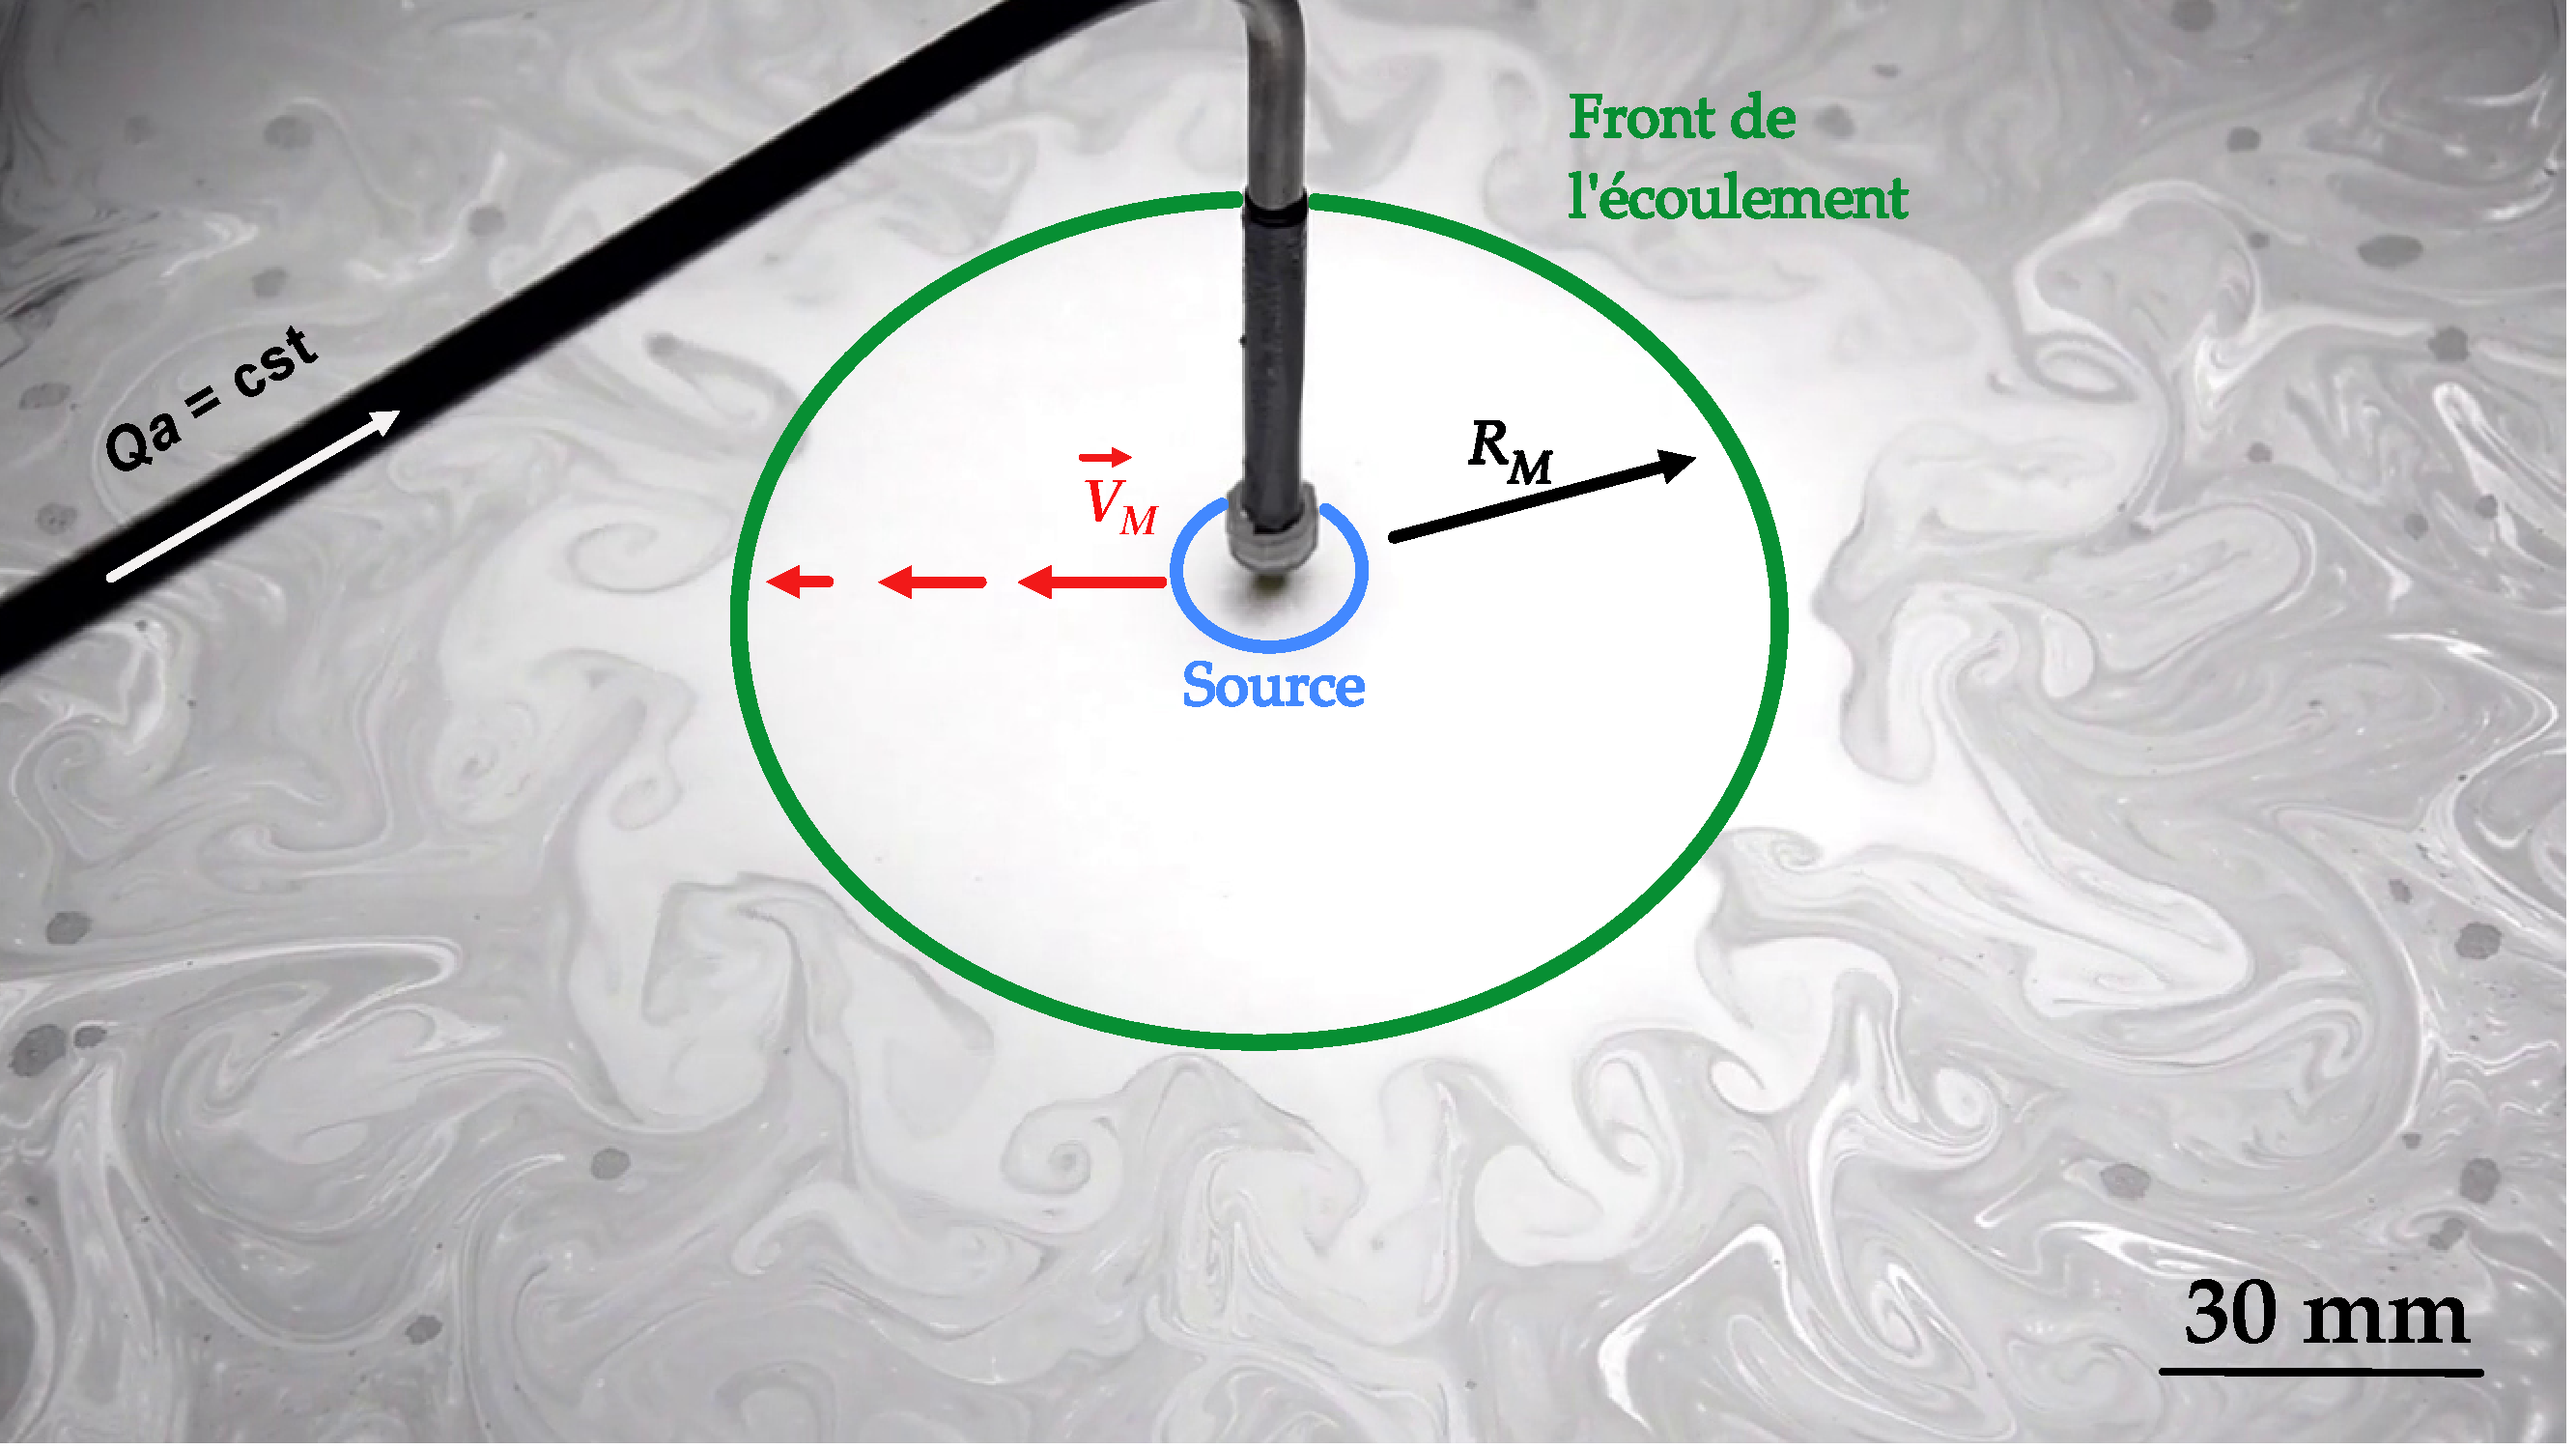
\includegraphics[width=1.1\textwidth]{./figures/Ecoulement_Marangoni_2.pdf}
        \end{figure}
      \end{minipage}\hfill
        \begin{minipage}{.45\textwidth}
          \centering
          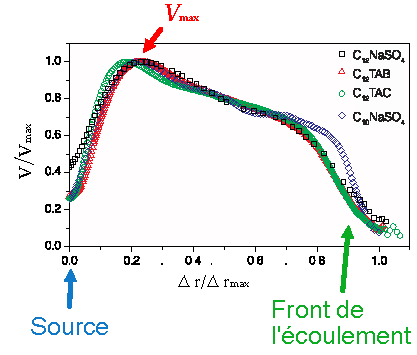
\includegraphics[scale=.8]{./figures/profil_vitesse_matthieu.pdf}
        \end{minipage}
    \end{frame}
    
    % \begin{frame}{1.5. Caractérisation de l'écoulement solutocapillaire}
    %     \begin{figure}
    %         \centering
    %         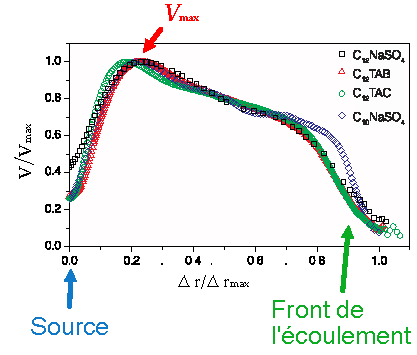
\includegraphics[scale=1]{./figures/profil_vitesse_matthieu.pdf}
    %     \end{figure}
    %     \footnote{[Roche 2014]}
    % \end{frame}

    \begin{frame}{1.5. Caractérisation de l'écoulement de Marangoni}
        \begin{ombredef}
            \begin{defi}
              \noindent\textbf{Rayon maximal stationnaire de l'écoulement de Marangoni soluto-capillaire:}\bigskip
                \begin{equation}
                    R_{\rm max}^{a} \propto \left(\frac{Q}{c^{*}}\right)^{3/4}\left(\frac{\eta\rho}{\Delta\gamma^2 D^3}\right)^{1/8}.
                \end{equation}
          
                \noindent \textbf{Vitesse maximale de l'écoulement de Marangoni soluto-capillaire:}\bigskip
                \begin{equation}
                V_{\rm max}^{a}\propto\left(\frac{c^{*}\Delta\gamma^3}{Q}\right)^{1/4}\left(\frac{D}{(\eta\rho)^3}\right)^{1/8}.
                \end{equation}
          \end{defi}
        \end{ombredef}
        \footnote{[Le Roux 2016]]} 
    \end{frame}


    \section{Génération de vorticité}

\begin{frame}{1.6. Structure de l'écoulement en fonction de l'épaisseur d'eau $h$}
    \begin{figure}
        \centering
        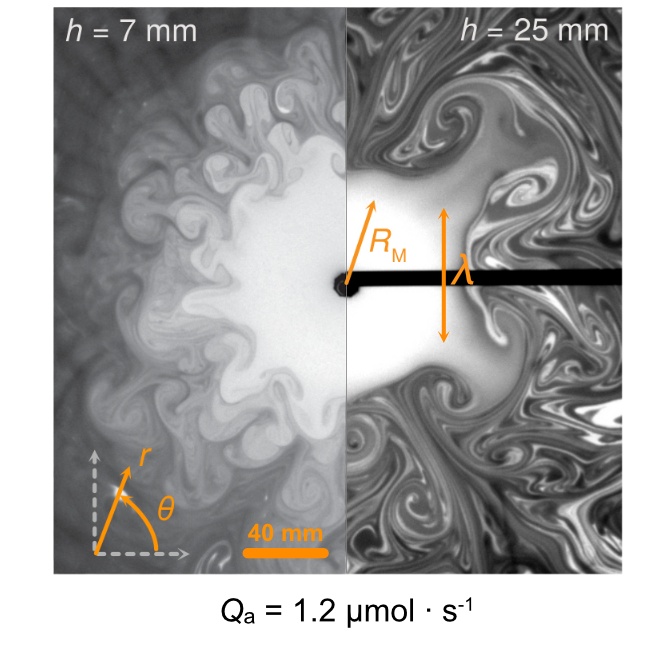
\includegraphics[width = .5\textwidth]{./figures/Marangoni_flow_emulsion_Qa1p2mumolL_h7mm_h25mm.png}
    \end{figure}    
\end{frame}


\begin{frame}{I.7. Longueur d'onde en fonction de $h$ et $Qa$}
    \begin{figure}[t]
        \centering
        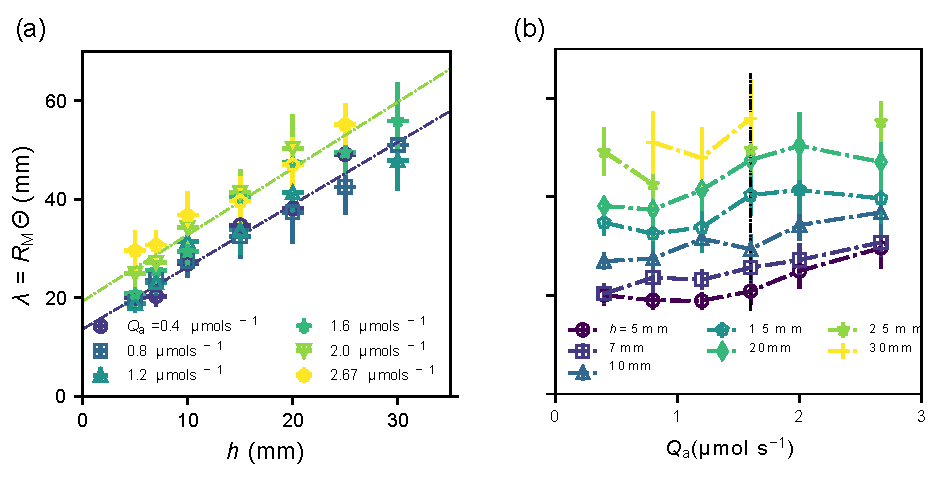
\includegraphics[width=.85\textwidth]{./figures/Lambda_measurement_1.pdf}
    \end{figure}
    \vspace{-.8cm}
    
    \hspace{1cm}\begin{minipage}{6cm}
        \begin{ombretheo}
            \begin{theo}
                \[\lambda \propto h\]
            \end{theo}
        \end{ombretheo}
    \end{minipage}
    \hspace{.4cm}\begin{minipage}{6cm}
        \begin{ombretheo}
            \begin{theo}
                \[\lambda(Q_{\rm a}) \sim \rm constante\]
            \end{theo}
        \end{ombretheo}
    \end{minipage}
\end{frame}

\begin{frame}{I.8. Dispositif experimental de PIV 3D}
    \begin{figure}
        \centering
        %\resizebox{.5\textwidth}{!}{\input{./figures/DispositifPIV.pdf_tex}}
        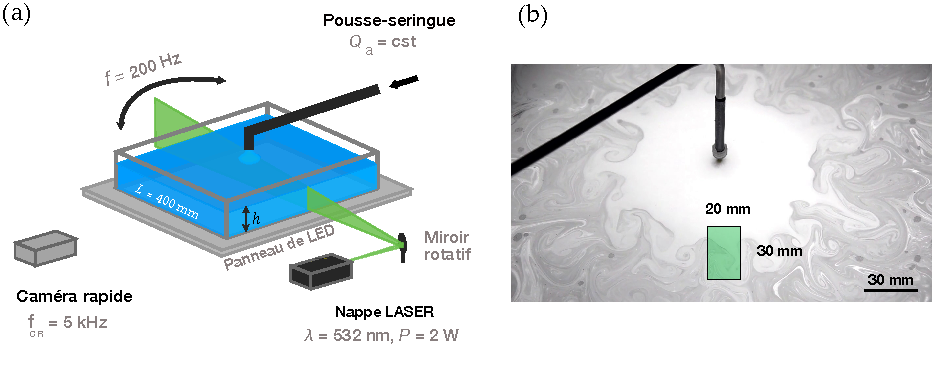
\includegraphics[width=1\textwidth]{./figures/DispositifPIV_v2.pdf}
    \end{figure}
    
    %Déplacement d'une particule entre un aller retour de la nappe LASER $dr\approx 40~\rm \upmu m < 1~\rm mm$ = taille d'une boîte de corrélation 
\end{frame}

\begin{frame}{I.9. Mesure du champ de vitesse et de vorticité ($h=15~\rm mm,~~Q_{\rm a} = 1.2~\rm \upmu mol\cdot s^{-1}$)}
    \begin{figure}[t]
        \centering
        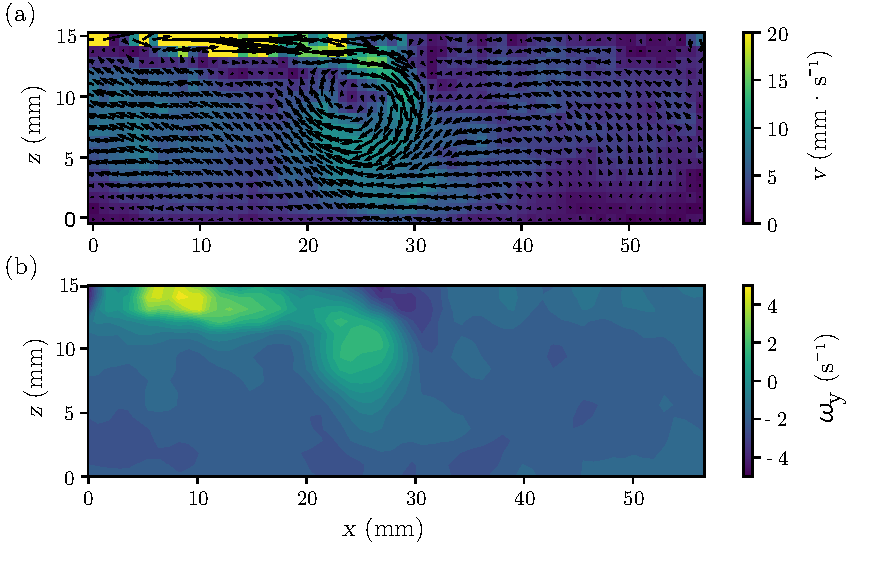
\includegraphics[scale=.8]{./figures/rolling_vortex_velocity_vorticity_v2.pdf}
    \end{figure}
\end{frame}


% \begin{frame}{I.9. Diaporama de la vorticité du tourbillon ($h=15~\rm mm,~~Q_{\rm a} = 1.2~\rm \upmu mol\cdot s^{-1}$)}
%     \begin{figure}
%         \centering
%         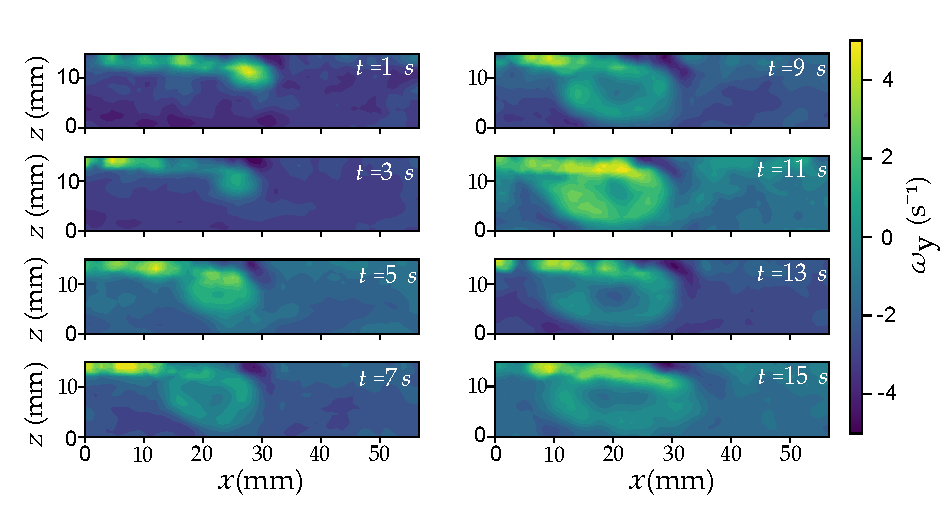
\includegraphics[scale=0.85]{./figures/Diaporama_vorticite.pdf}
%     \end{figure}
% \end{frame}

\begin{frame}{I.9. Deux phénomènes en jeu}
    \begin{multicols}{2}
        \begin{figure}
            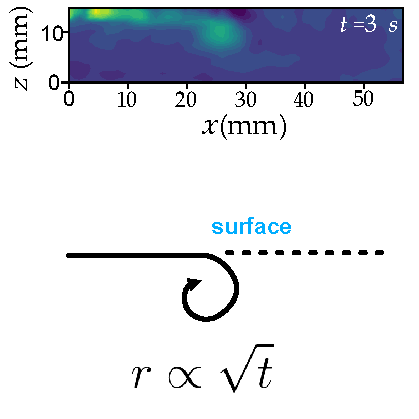
\includegraphics[scale=1]{./figures/schema_enroulement_proche_surface.pdf}
        \end{figure}
        \begin{figure}
            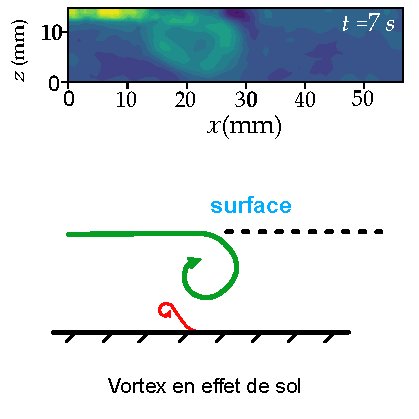
\includegraphics[scale=1]{./figures/schema_enroulement_proche_surface_2.pdf}    
        \end{figure}
    \end{multicols}

\end{frame}


\begin{frame}{I.10. Modèle de la croissance du tourbillon}


    \begin{columns}
      \begin{column}{.55\textwidth}
        À partir d'un bilan de masse entre le tourbillon et la couche limite:
    \begin{ombretheo}
        \begin{theo}
            \textbf{Croissance du tourbillon $r\propto \sqrt{t}$}
    \begin{equation}
            r(t)=\delta\sqrt{1+\frac{vt}{2\pi\delta}}\nonumber.
    \end{equation}
\end{theo}
\end{ombretheo}
    
    \textbf{Paramètres:}

    \begin{itemize}
        \item $\delta$ épaisseur de la couche limite : ajusté;
        \item $\delta \in [1,3]~\rm mm$     
        \item $v$ vitesse de l'écoulement de Marangoni: mesuré.
    \end{itemize}

      \end{column}
      \begin{column}{.5\textwidth}
        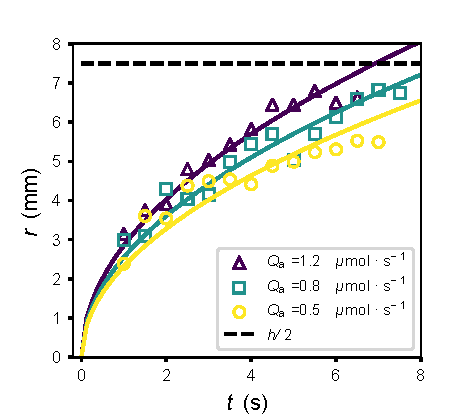
\includegraphics[width=1\textwidth]{./figures/Rayon_vs_modele.pdf}
      \end{column}
    \end{columns}
\end{frame}

\begin{frame}{I.11. Vortex en effet de sol}
  \vspace{-.5cm}
  \begin{figure}[t]
      \centering
      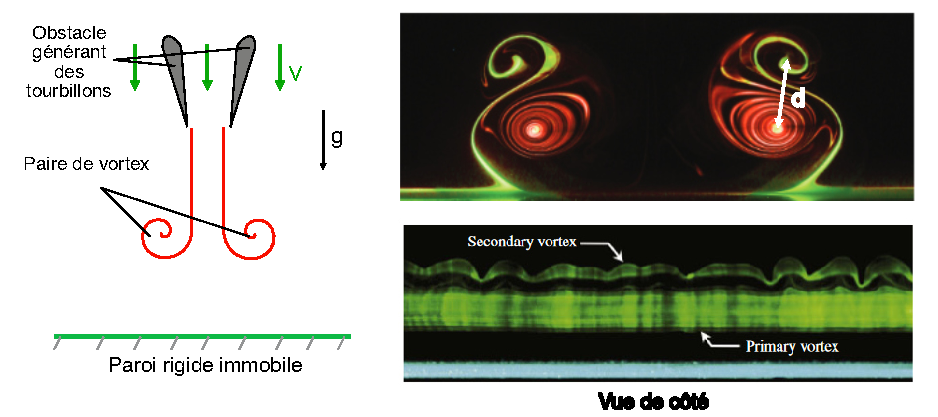
\includegraphics[scale=.9]{./figures/VortexInGroundEffect_vf_n1.pdf}\footnote{[Leweke 2016, Harris 2012]}
  \end{figure}
\end{frame}



% \begin{frame}{2.12. Contamination de la surface}
%     \begin{figure}
%         \centering
%         \resizebox{.7\textwidth}{!}{\input{./figures/ContaminationVortex.pdf_tex}}
%     \end{figure}
% \end{frame}

\begin{frame}{Conclusion partielle : génération de vorticité}
    \begin{enumerate}
        \item La génération de vorticité intefaciale provient d'une instabilité de vortex en effet de sol
        \item Il nous manque encore une preuve directe de la seconde génération de vorticité;
        \end{enumerate}
        \begin{figure}
            \centering
            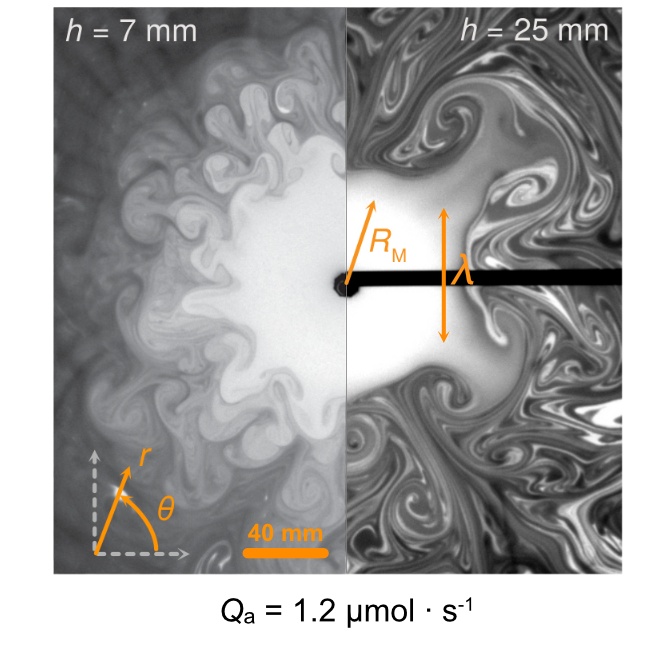
\includegraphics[width = .4\textwidth]{./figures/Marangoni_flow_emulsion_Qa1p2mumolL_h7mm_h25mm.png}
        \end{figure} 
\end{frame}

\section{Propulsion par effet Marangoni}

\begin{frame}{II.1. Dispositif Experimental}
  \begin{minipage}{.6\linewidth}
    \begin{figure}
        \centering
        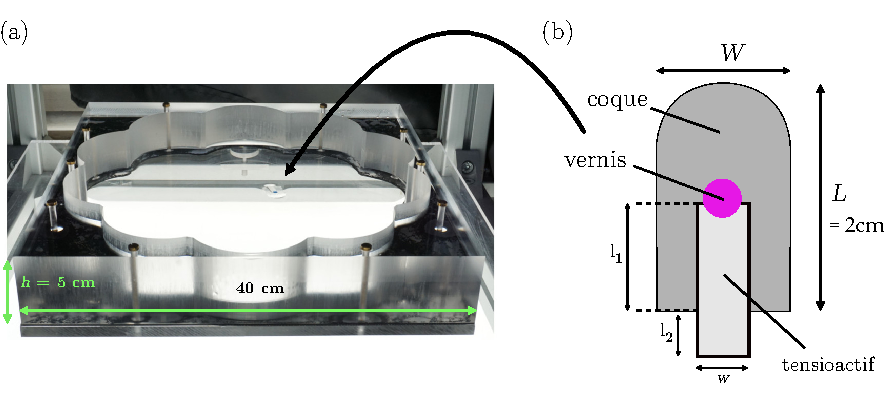
\includegraphics[width=.9\linewidth]{./figures/Dispositif_Exp_Bateau_Marangoni_v2.pdf}\\
        \movie{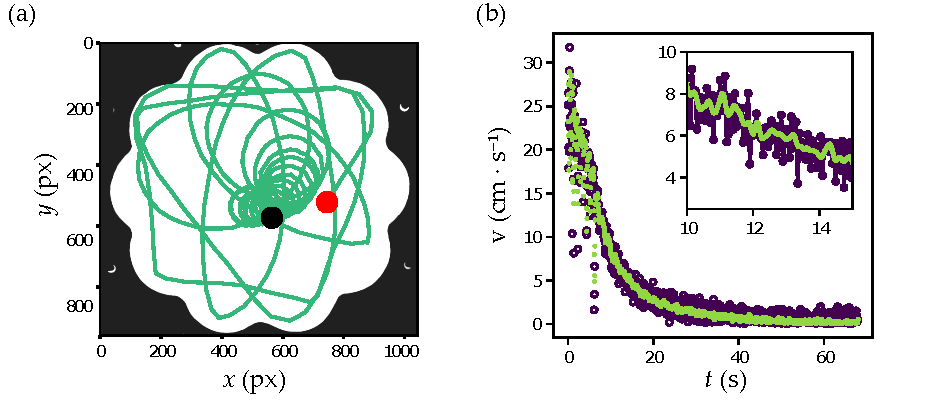
\includegraphics[width=\linewidth]{./figures/Trajectoire_bateau_2.pdf}}{./videos/new_bateau_cuve_fleurie_20hz.avi}
    \end{figure}
  \end{minipage}
  \begin{minipage}{.35\linewidth}
    \begin{table}
      \centering
      \resizebox{1\linewidth}{!}{
      \begin{tabular}{ccc}
        \hline \hline
        Tensioactif & CMC ($\rm mmol\cdot L^{-1}$) & $v_{\rm max}$ ($\rm cm\cdot s^{-1}$)\\ \hline \hline
        HTAC & $1.3$ & $28.1\pm 1.1$ \\
        TTAB & $3.6$ & $26.5\pm 1.5$\\
        DoTAB & $15.4$ &  $25.2 \pm 1.6$ \\
        DeTAB & $62.5$ & $22.2\pm 1.1$\\ \hline \hline 
      \end{tabular}}
      \caption{Tableau des vitesses initiales}
    \end{table}
    \begin{ombretheo}
      \begin{theo}
        Plus le tensioactif est soluble moins la vitesse du bateau est grande.
      \end{theo}
    \end{ombretheo}
  \end{minipage}
\end{frame}

\begin{frame}{TP proposé à des classes de niveau seconde : effet de la pollution des eaux}
  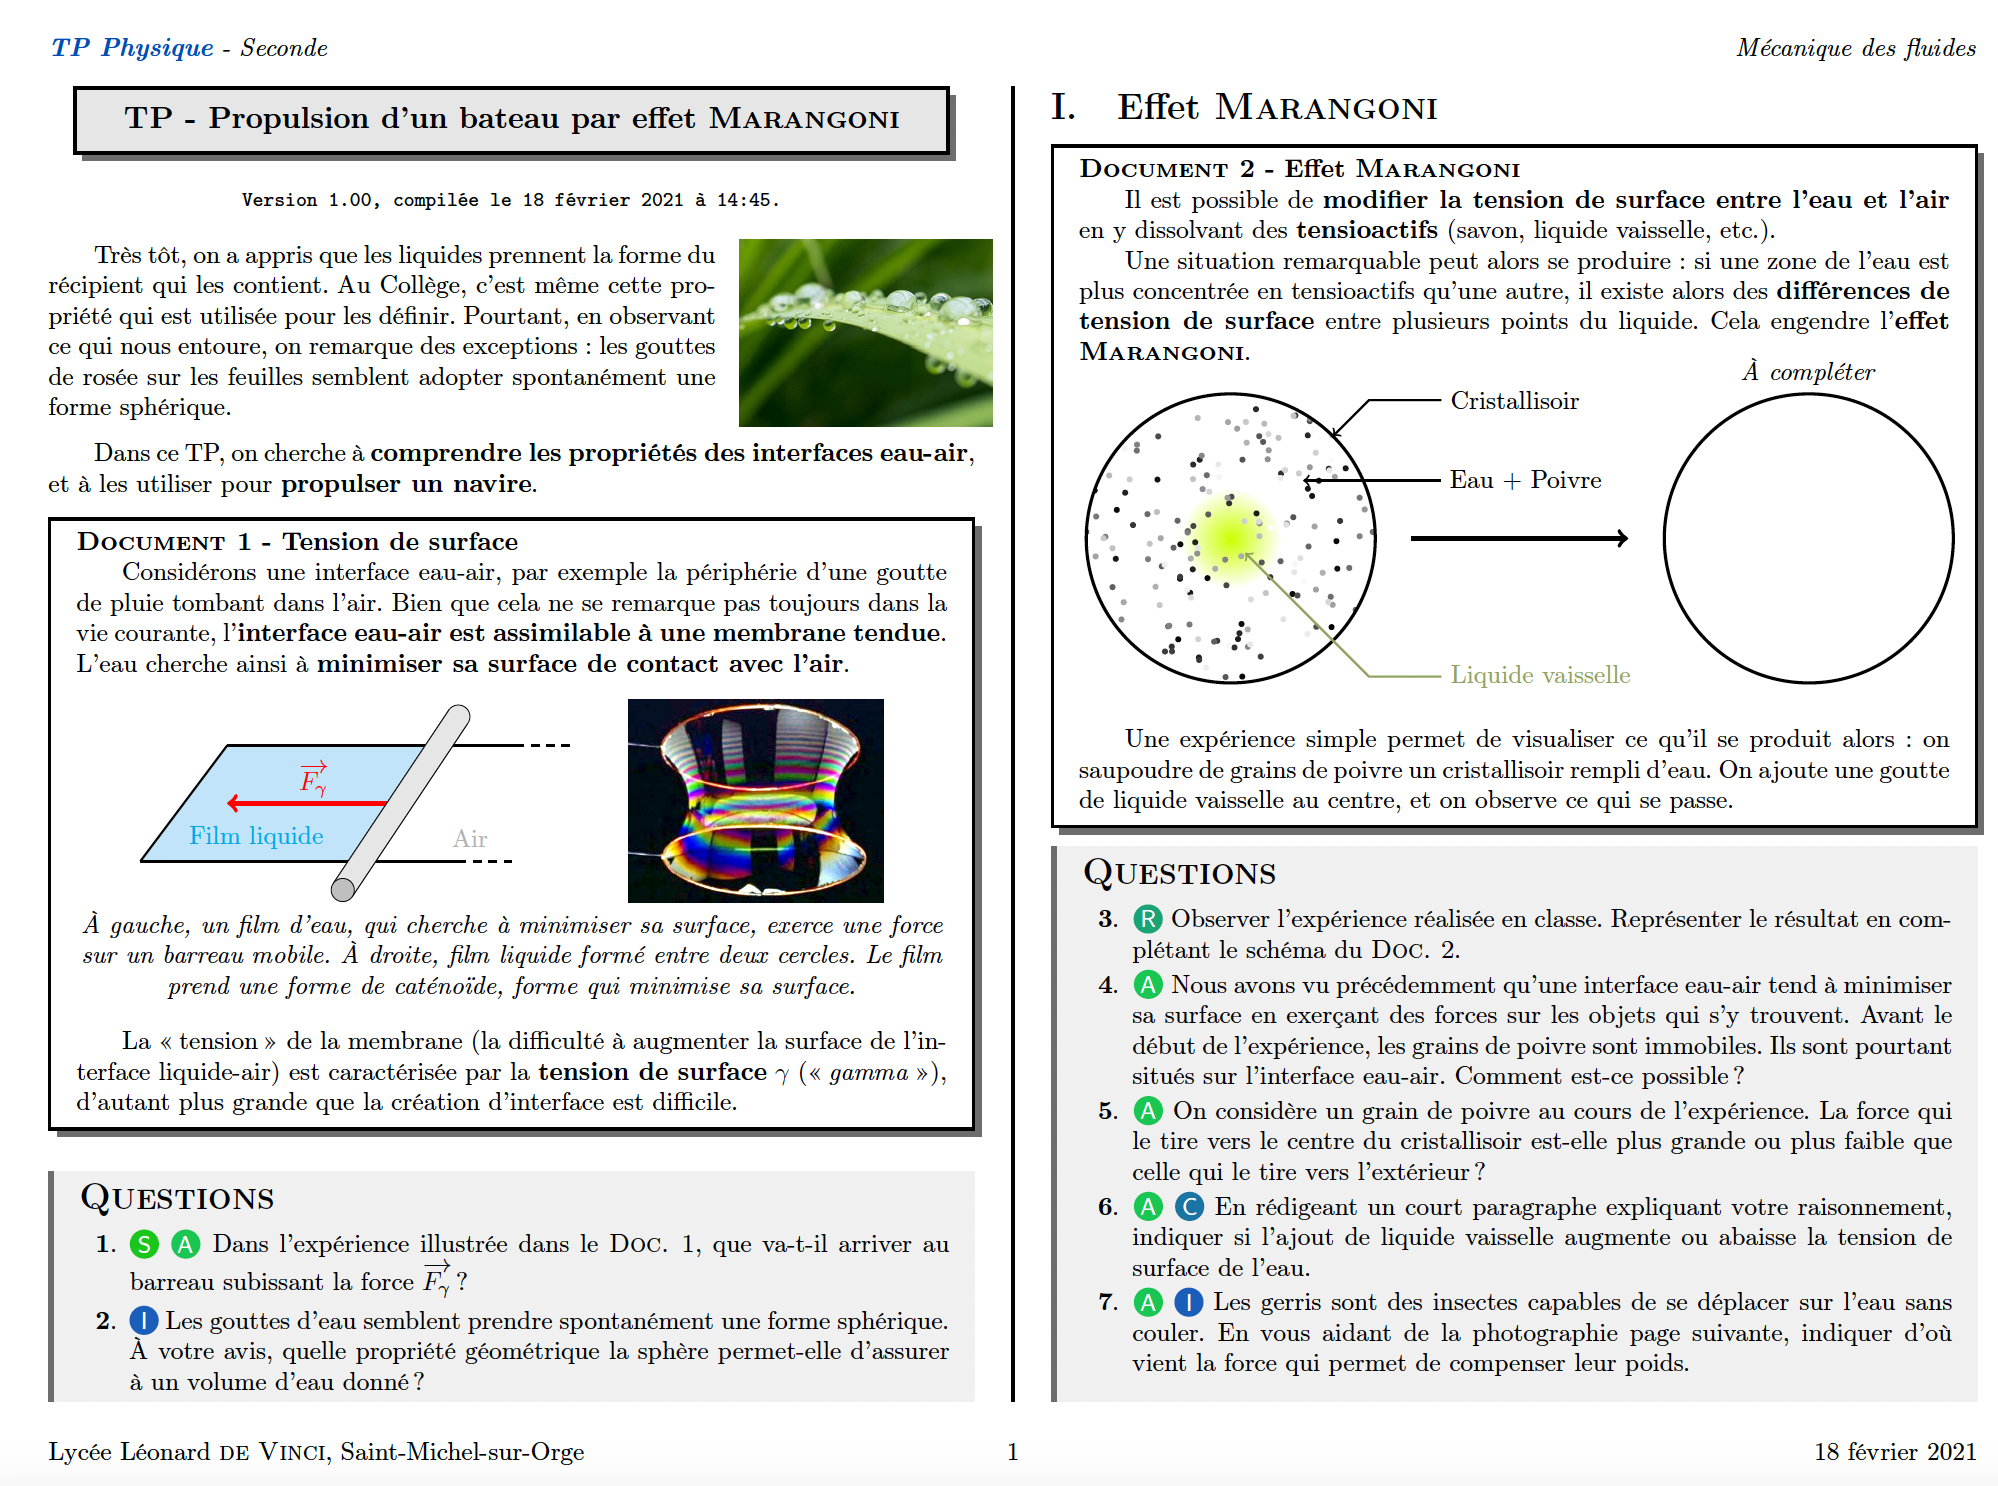
\includegraphics[width=\linewidth]{TP_Marangoni1.png}
\end{frame}

\begin{frame}{TP proposé à des classes de niveau seconde : effet de la pollution des eaux}
  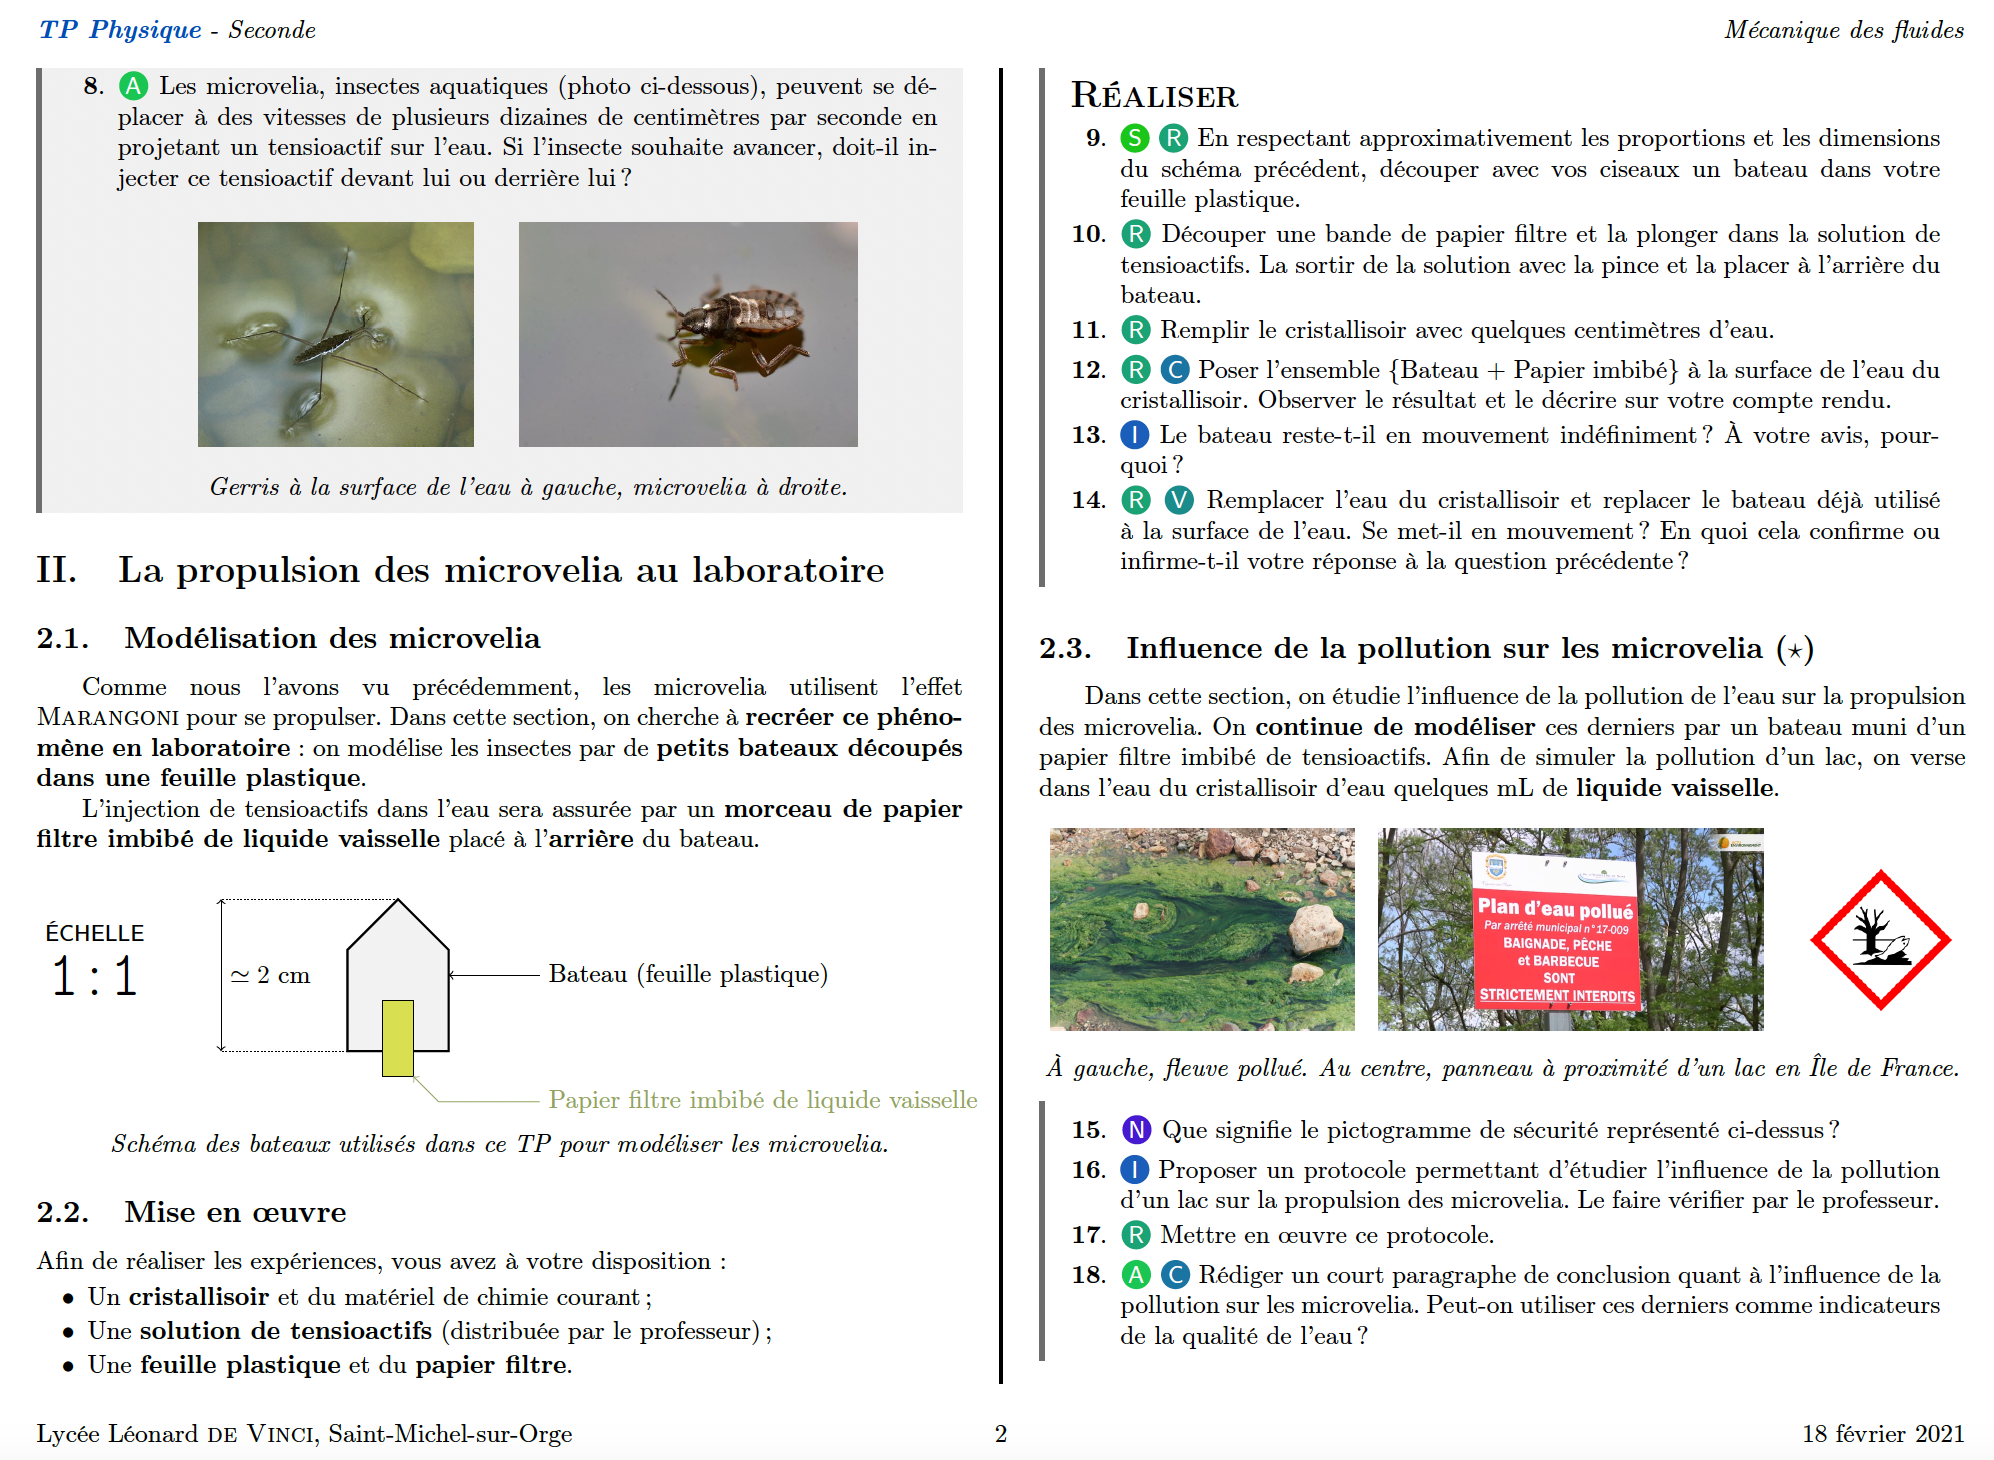
\includegraphics[width=\linewidth]{TP_Marangoni2.png}
\end{frame}
% \begin{frame}{II.2. Trajectoire du bateau et mesure de la vitesse au cours du temps}
%     \begin{figure}
%         \centering
%         \movie{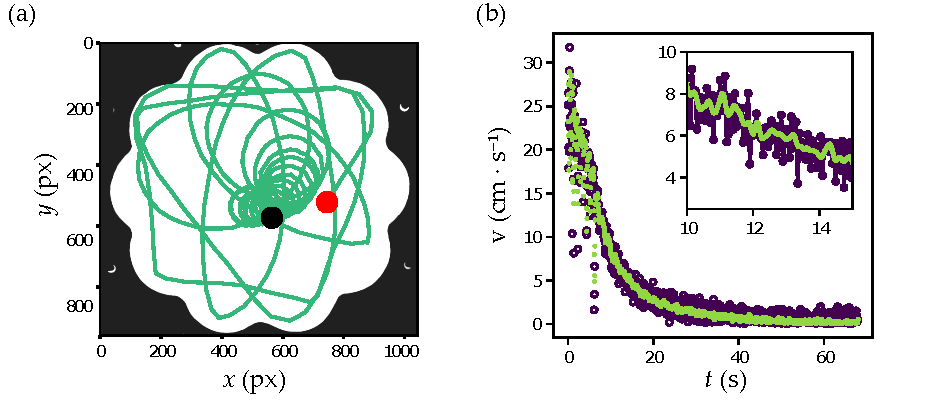
\includegraphics[scale=0.8]{./figures/Trajectoire_bateau_2.pdf}}{./videos/new_bateau_cuve_fleurie_20hz.avi}
%     \end{figure}
% \end{frame}


\begin{frame}{II.2. Modélisation de la propulsion du bateau}
    \begin{minipage}{6cm}
        \textbf{Bilan des forces:}\bigskip
        \begin{equation}
            m\frac{d\vv{v}}{dt} = \sum_i \vv{F_{\rm i}}\nonumber
        \end{equation}

        Le bateau se déplace dans le plan de la surface de l'eau (Oxy): 

        \begin{equation}
            m\frac{d\vv{v}}{dt} = F_{\rm M} - F_{\rm D}
        \end{equation}

    \end{minipage}
    \begin{minipage}{7cm}  
        \begin{figure}
            \centering
            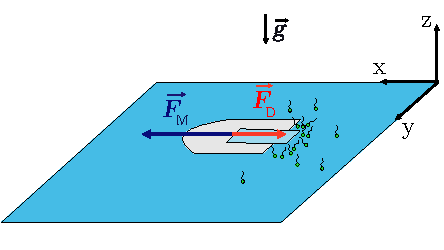
\includegraphics[scale=1]{./figures/SchemaModeleBateau.pdf}
            %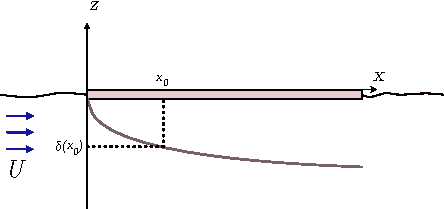
\includegraphics[scale=.8]{./figures/couchelimitesketch.pdf}
        \end{figure}
    \end{minipage}
\end{frame}


\begin{frame}{II.3. Calcul de la force de frottement}


    \begin{multicols}{2}
      \textbf{Reynolds de nos bateaux de Marangoni:}
      \[ Re \approx 10^3 \] 
    
      \textbf{Friction de peau pour :}
      $$10^{2}<\rm Re\approx 10^{3}<<10^{6}$$
    
      \begin{ombredef}
        \begin{defi}
      \begin{equation}
        F_{\rm D} = 0.664\rho W\sqrt{\nu L}v^{3/2}=\beta v^{3/2}.\footnote{D'après G. Pucci et.al. 2019}
        \end{equation}
        \end{defi}
    \end{ombredef}
    
    \begin{figure}
      \centering
      %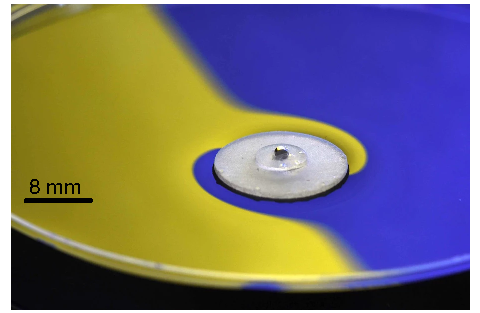
\includegraphics[width=.4\textwidth]{./figures/Pucci.pdf}
      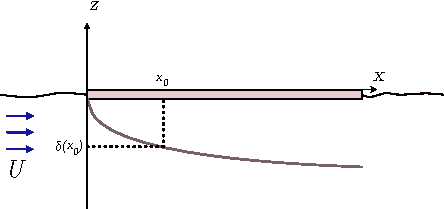
\includegraphics[scale=.8]{./figures/couchelimitesketch.pdf}
    \end{figure}
    \end{multicols}
    \end{frame}

    
\begin{frame}{II.4. Équation à résoudre}
    \begin{ombredef}
      \begin{defi}
        \noindent\textbf{Équation à résoudre:}
        \begin{equation}
          m\frac{dv(t)}{dt} =\alpha L\Delta\gamma(c_0)\rm f(t)-\beta v(t)^{3/2}.
        \end{equation}
      \end{defi}
    \end{ombredef}
    \begin{enumerate}
      \item Nous résolvons l'équation stattionaire $dv(t)/dt = 0$, $f(t)=1$:
       $$0 = \alpha L\Delta\gamma(c_0) - \beta v_0^{3/2},$$
      \item Nous résolvons l'équation à chaque instant $dv(t)/dt \neq 0$ $f(t)=\exp(-t/\tau_M)$:
      $$m\frac{dv(t)}{dt} =\alpha L\Delta\gamma(c_0) {\rm e}^{-\dfrac{t}{\tau_{\rm M}}}-\beta v(t)^{3/2}.$$
    \end{enumerate}
    \end{frame}

    % \begin{frame}{3.5. Comparaison avec la littérature}
    %     \begin{table}[ht!]
    %       \centering
    %       \begin{tabular}{c|c|c|c}
    %         \hline \hline
    %         Tensio-actifs & $\Gamma_{\rm max}~\rm (mol\cdot m^{-2})$ & $K_{\rm L }~\rm (m^{3}\cdot mol^{-1})$ ajusté &$K_{\rm L }~\rm (m^{3}\cdot mol^{-1})$ Litt. \\ \hline \hline
    %         HTAC, $\rm C_{16}TAC$  & $3.4\cdot 10^{-6}$ & $4.4$ &  \\ 
    %         TTAB, $\rm C_{14}TAB$  & $3.3\cdot 10^{-6}$& $3.2$ &  $1.2$ \\ 
    %         DoTAB, $\rm C_{12}TAB$  & $2.9\cdot 10^{-6}$ & $2.7$ & \\ 
    %         DeTAB, $\rm C_{10}TAB$  & $2.8\cdot 10^{-6}$ & $1.1$ &\\  \hline
    %       \end{tabular}
    %       \label{TABLE:Paramv0}
    %     \end{table}\footnote{\cite{Nguyen2017}}
    %   \end{frame}


    \begin{frame}{II.5. Résolution de l'équation stationnaire}
\begin{minipage}{.5\textwidth}
  Si on considère le cas stationnaire de cette équation il vient:
  \begin{equation}
      \beta v_0^{3/2} = \alpha L\Delta\gamma(c_0).\label{eq:stationnaire}
    \end{equation}
    
    
    En isolant d'un côté de l'équation la vitesse $v_0$ il vient directement l'expression de la vitesse initiale en fonction de la concentration:
   \begin{ombretheo}
    \begin{theo}
    \begin{equation}
      v_0(c_0)=\left(\frac{\alpha RT\Gamma_{\rm max}}{0.664\rho l}\sqrt{\frac{L}{\nu}}\ln(1+K_{\rm L}c_0)\right)^{2/3}.
      \label{eqn:v0}
    \end{equation}
  \end{theo}
\end{ombretheo}
\end{minipage}\hfill
\begin{minipage}{.45\textwidth}
  \begin{figure}
    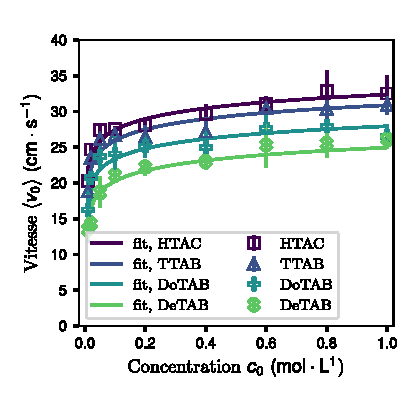
\includegraphics[width=1\textwidth]{./figures/Bateau_v0_final.pdf}
\end{figure}
\end{minipage}
  \end{frame}
  
  
\begin{frame}{Conclusion Partielle: Propulsion des bateaux de Marangoni}
    \begin{enumerate}
    \item La propulsion est sensible aux propriétés du tensioactif.
    \item Modèle naïf qui décrit bien le système.
    \item Description de la vidange du réservoir de tensioactif dans le temps et étalement des molécules.
    \end{enumerate}
    \begin{figure}
      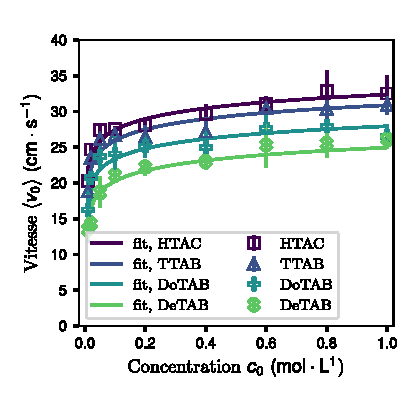
\includegraphics[width=.4\textwidth]{./figures/Bateau_v0_final.pdf}
  \end{figure}
\end{frame}
  
\begin{frame}{Parcours de formation à et par l'enseignement}
  \centering
  \begin{minipage}{.35\linewidth}
  \centering
  
\includegraphics[width=.25\linewidth]{./figures/vulgarisation.jpg}\smallskip
  
  \textbf{\large Vulgarisation}\smallskip
  
  \textbf{Fête de la science}\smallskip

  Université de Paris Cité - 2019\smallskip
  
  \textbf{Projet de vulgarisation : Marangoni}\smallskip

  \url{https://dgxy.link/Marangoni} - 2018-2021\smallskip
  


  \textbf{Conférence au lycée 2nd/CPGE}\smallskip
  
  Lycée Lépérouse Kerichen - Brest - 2019\smallskip

  Lycée Léonard de Vinci - Saint-Michel sur Orge - 2020
  
  \end{minipage}\hfill
  \begin{minipage}{.25\linewidth}
    \centering
  
\includegraphics[width=.25\linewidth]{./figures/etudes.jpg}\smallskip
  
  \textbf{\textcolor{red}{Préparation à l'agrégation de physique au centre de Rennes }}\smallskip
  
  2023-2023 \smallskip
  
  \textbf{\textcolor{red}{Formation à l'INSPE de Bretagne}}\smallskip
  
  2023-2024
  
  \end{minipage}\hfill
  \begin{minipage}{.35\linewidth}
    \centering
  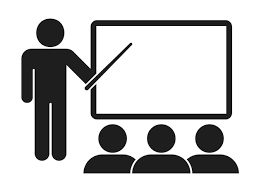
\includegraphics[width=.25\linewidth]{./figures/enseignement.jpg}\smallskip
  
  
  \textbf{\textcolor{blue}{Enseignement}}\smallskip
  
  \textbf{Cours/TDs de physique en PASS et L1 SVT}\smallskip
  
Université Paris Cité - 128 heures - 2018-2021 \smallskip

\textbf{Professeur stagiaire de physique chimie}\smallskip
  
Lycée Jean Guéhenno - Fougères - 2023-2024.

  \end{minipage}
\end{frame}
\section{Annexes}


\begin{frame}{Longueur d'onde en fonction de $h$, Méthode expérimentale}
  \begin{figure}
      \centering
      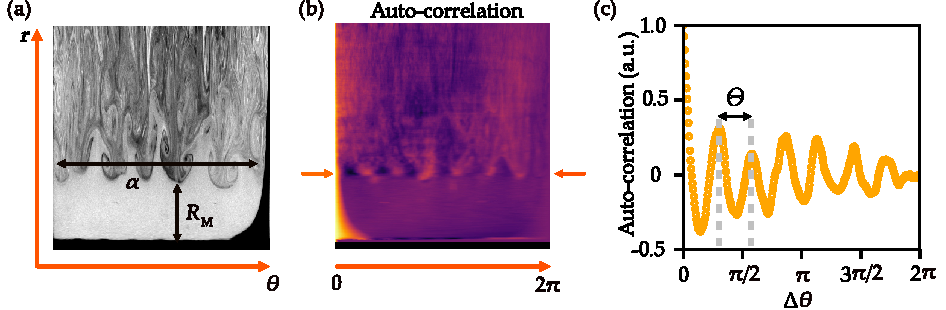
\includegraphics[scale=.85]{./figures/Methode_analyse_lambda.pdf}
      %\resizebox{.65\textwidth}{!}{\input{./figures/TraitementEmulsion.pdf_tex}}
  \end{figure}

  \begin{ombredef}
      \begin{defi}
          \begin{multicols}{2}
          \begin{itemize}
              \item[$\bullet$]{\textbf{Distance angulaire moyenne:}}
                \begin{equation}
                  \Theta = \frac{\alpha}{N}.
                  \label{eq:Theta}
                \end{equation}
              \item[$\bullet$] {\textbf{Distance entre paires de vortexs:}}
                \begin{equation}
                  \lambda = R_{\rm M}\Theta.
                  \label{eq:lambda}
                \end{equation}
              \end{itemize}
          \end{multicols}
      \end{defi}
  \end{ombredef}
\end{frame}

\begin{frame}{Contrôle de l'émission des vortex}
  \begin{figure}
      \centering
      
      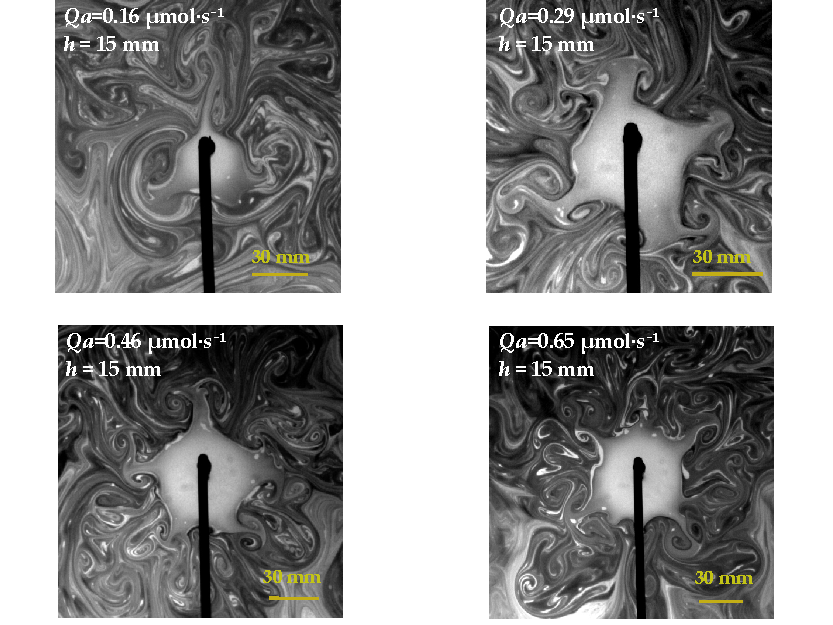
\includegraphics[scale=.7]{./figures/Instabilite.pdf}
      %\includegraphics[scale=.8]{./figures/Instabilite_surface_0.pdf}
  \end{figure}
\end{frame} 

\begin{frame}{Modèle de la croissance du tourbillon}
  \begin{columns}
    \begin{column}{.5\textwidth}
       \begin{enumerate}
      \item Flux de masse entrant dans le vortex:
      $$j_{\rm m}=\rho v \delta,~\text{avec}~ \delta = \sqrt{\frac{\nu R}{v}};$$
      \item Masse du vortex: 
      $$m(t)=\pi r^{2}(t)\rho.$$
      \end{enumerate}
      \textbf{Conservation de la masse:} 
      \[ \dot{m}=j_{\rm m}~  \implies~ 2\pi \rho r\dot{r}=v\rho\delta. \]
      
      \vspace{-.5cm}\begin{ombretheo}
          \begin{theo}
      La solution de l'équation est:
      \begin{equation}
          r(t)=\delta\sqrt{1+\frac{vt}{2\pi\delta}}.
      \end{equation}
  \end{theo}
\end{ombretheo}
    \end{column}
    \begin{column}{.55\textwidth}
      \centering
      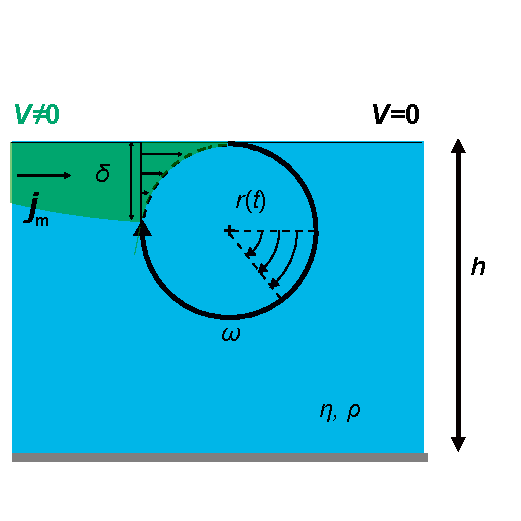
\includegraphics[width=.8\textwidth]{./figures/Schema_enroulement_v3.pdf}
    \end{column}
  \end{columns}
\end{frame}

\begin{frame}{Profil du vortex de type Rankine}
  \begin{figure}
    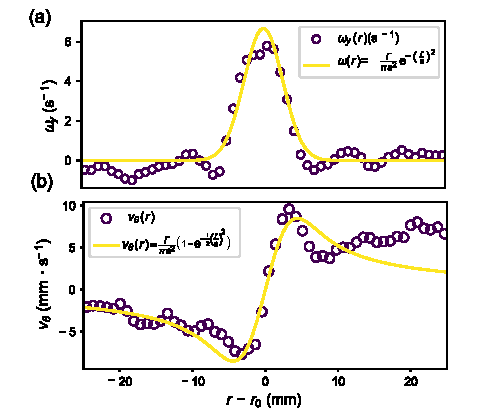
\includegraphics[width=.5\textwidth]{Vorticityprofile_v2.pdf}
  \end{figure}
\end{frame}

\begin{frame}{Vortex en effet de sol}
  \vspace{-.5cm}
  \begin{figure}[t]
      \centering
      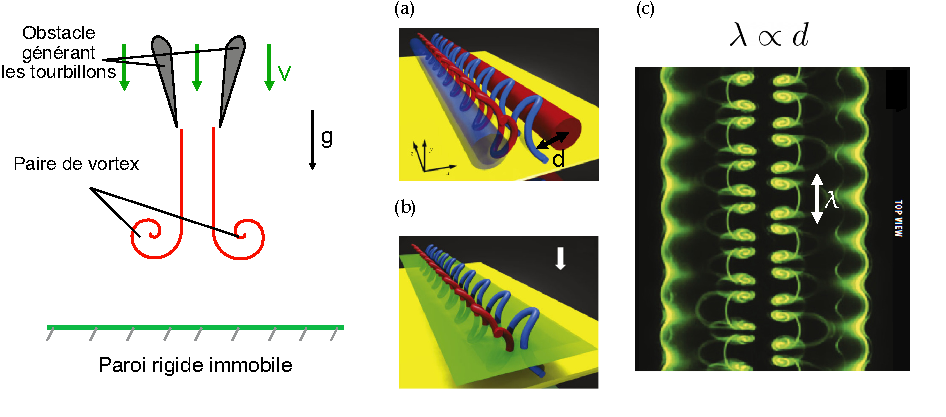
\includegraphics[scale=.9]{./figures/VortexInGroundEffect.pdf}\footnote{[Leweke 2016, Harris 2012]}
  \end{figure}
\end{frame}


\begin{frame}{Processus de reconnexion de la vorticité}
  \begin{figure}
      \resizebox{.9\textwidth}{!}{\input{./figures/MecansimeReconnexionWillert97.pdf_tex}}
  \end{figure}\footnote{D'après [Willert 1997]}
\end{frame}

\begin{frame}{Processus de reconnexion de la vorticité}
  \begin{figure}[!ht]
      \centering
      %\includegraphics{./figures/Schema_vortex_impact_surface_libre.pdf}
      \resizebox{.75\textwidth}{!}{\input{./figures/WillertGharib97_manips.pdf_tex}}
     \footnote{D'après [Willert 1997]}
    \end{figure}
  \end{frame}


  
  \begin{frame}{Comparaison entre l'expérience et le modèle}
    \vspace{-.5cm}
      \begin{figure}
          \centering
          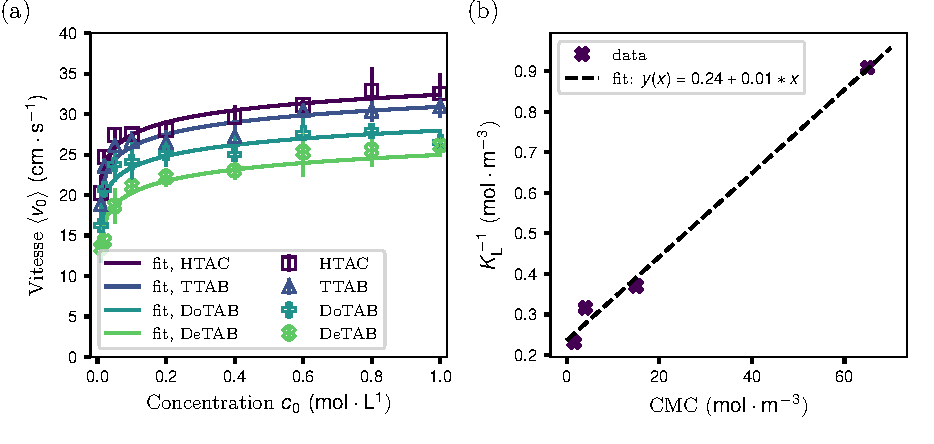
\includegraphics[scale=.7]{./figures/Vitesse_initiale_versus_concentration_modele.pdf}
      \end{figure}
      \vspace{-.5cm}
      \hspace{1.5cm}\begin{minipage}{4cm}
        \begin{ombretheo}
          \begin{theo}
            $v_0$ augmente avec $c_0$
          \end{theo}
        \end{ombretheo}
      \end{minipage}
      \hspace{3.cm}
      \begin{minipage}{5cm}
        \begin{ombretheo}
          \begin{theo}
            $K_L^{-1}$ augmente avec la $CMC$
          \end{theo}
        \end{ombretheo}
      \end{minipage}
  \end{frame}
  
  \begin{frame}{Génération de vagues}
    \begin{figure}[!ht]
        \centering
        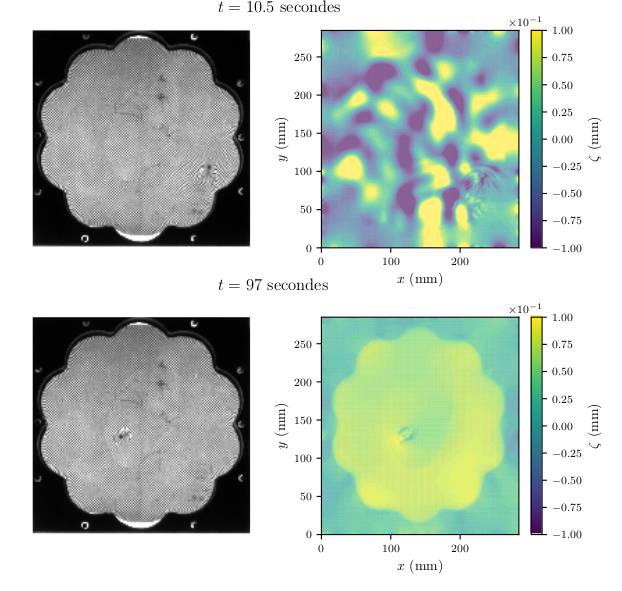
\includegraphics[scale=.5]{./figures/Generation_de_vagues.png}
        \caption{Déformation de surface dans la cuve fleurie}
  \end{figure}
\end{frame}


\begin{frame}{Variation de la vitesse pour différents tensioactifs}
  \begin{minipage}{8cm}
      \begin{figure}[!ht]
          \centering
          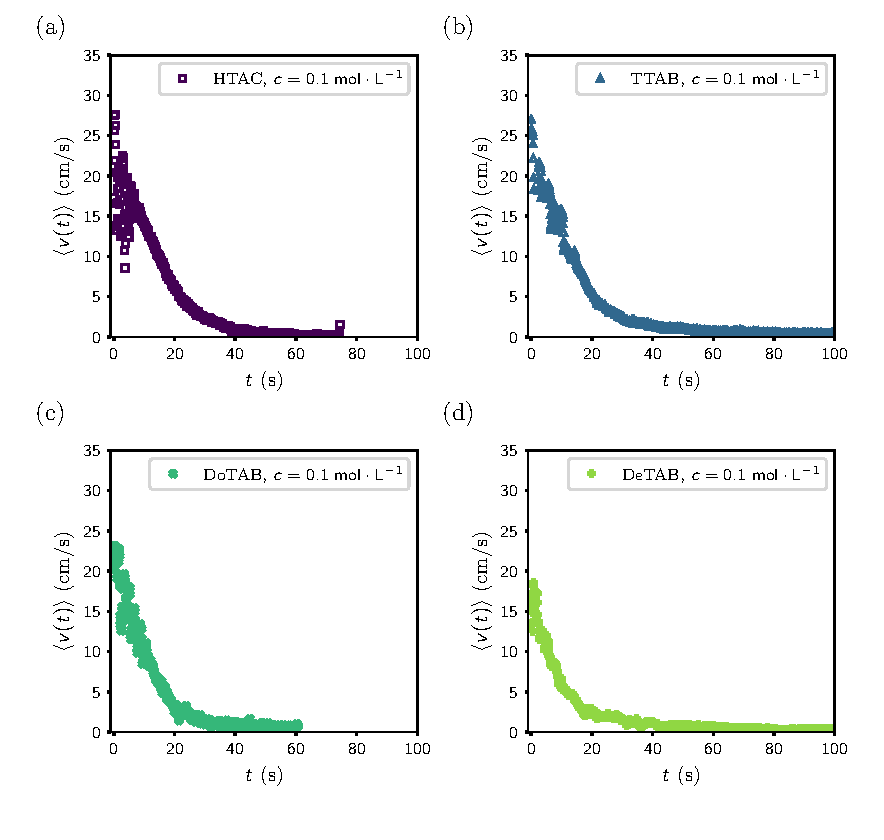
\includegraphics[scale=0.55]{./figures/Deceleration_vitesse_faible_concentration.pdf}
      \end{figure}
  \end{minipage}
  \begin{minipage}{5cm}
      \begin{table}
          \centering
          \resizebox{1\textwidth}{!}{
          \begin{tabular}{ccc}
            \hline \hline
            Tensioactif & CMC ($\rm mmol\cdot L^{-1}$) & $v_{\rm max}$ ($\rm cm\cdot s^{-1}$)\\ \hline \hline
            HTAC & $1.3$ & $28.1\pm 1.1$ \\
            TTAB & $3.6$ & $26.5\pm 1.5$\\
            DoTAB & $15.4$ &  $25.2 \pm 1.6$ \\
            DeTAB & $62.5$ & $22.2\pm 1.1$\\ \hline \hline 
          \end{tabular}}
          \caption{Tableau des vitesses initiales}
        \end{table}
        \begin{ombretheo}
          \begin{theo}
            Plus le tensioactif est soluble moins la vitesse du bateau est grande.
          \end{theo}
        \end{ombretheo}
  \end{minipage}
\end{frame}


\begin{frame}{Force de frottement par les vagues}
    \begin{minipage}{10cm}
            \begin{equation}
                F_{\rm vague} = \frac{F}{(2\pi)^2\rho}\int\mathrm{d}\vv{k}\left(\frac{ik|\phi(kb)^2\vv{k}}{\omega_0(k)^2-4\nu^2k^3q+(2\nu k^2-i\vv{k}\cdot\vv{v})^2}\right).
            \end{equation}
            \begin{itemize}
              \item $\gamma = 70\times 10^{-3}~\rm N\cdot m^{-1}$, et  $\eta = 1\times 10^{-3}~\rm Pa\cdot s$
                 $\frac{\gamma}{\eta} = 70~\rm m\cdot s^{-1}>> v_{\rm Marangoni~boat}$
                \item À faible vitesse ($v<\gamma/\eta$) 
                $F_{\rm vague}\approx\left(\frac{P}{\gamma b}\right)^{2}\eta v b;$ \checkmark
                \item À grande vitesse ($v>\gamma/\eta$) $F_{\rm vague}\approx \frac{P^2}{\eta v b}$
                \end{itemize}
    \end{minipage}
    \begin{minipage}{3cm}
            \begin{figure}
              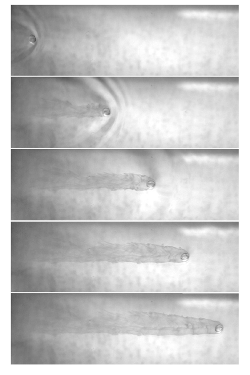
\includegraphics[scale=1]{./figures/Lemerrer.pdf}
            \end{figure}
    \end{minipage}

    \footnote{D'après [Le Merrer 2011]}
\end{frame}

\begin{frame}{Force de frottement par les vagues et friction de peau}
    \begin{minipage}{5cm}
        Comparaison du terme de friction de peau entre la coque du bateau et la surface de l'eau : 

        \[F_{\rm D} = \beta v^{3/2},\]

        par rapport au frottement par les vagues:

        \[F_{\rm vague}\approx\left(\frac{P}{\gamma b}\right)^{2}\eta v b.\]
        
    \end{minipage}
    \begin{minipage}{8cm}
            \begin{figure}[!ht]
            \centering
            \includegraphics[scale=1]{./figures/Forces_de_friction.pdf}
        \end{figure}
    \end{minipage}
\end{frame}


\begin{frame}{Force de propulsion}
  \textbf{Force de tension de surface entre l'avant et l'arrière du bateau:}
     
      \begin{equation}
        F_{\rm M} = \alpha L\Delta\gamma\left(c(r,t)\right).\nonumber 
      \end{equation}
      \begin{equation}
         F_{\rm M} = \alpha L \times \underbrace{\Delta\gamma_0(c_0)}_{\text{ Isotherme de Langmuir}}\times f(t)
    \end{equation}
    \textbf{Équation de surface de Gibbs}

    \begin{equation}
      d\gamma=-\Gamma_sd\mu_s\Rightarrow    d\mu_s=RT\ln c_s
    \end{equation}

    \begin{equation}
      \begin{array}{cc}
        d\gamma=-\left(\dfrac{RT}{c_s}\right)\Gamma_sd c & \Gamma_s=-\dfrac{1}{RT}\dfrac{d\gamma}{d\ln c_s}
      \end{array}
    \end{equation}


    \textbf{Isotherme de Langmuir:}
    \begin{equation}
      \begin{array}{cc}
        \Delta\gamma(c_0) = RT\Gamma_{\rm max}\ln{\left(1+K_{\rm L}c_0\right)} & \Gamma(c_0) = \Gamma_{\rm max}\frac{K_{\rm L}c_0}{1+K_{\rm L}c_0}.
      \end{array}
    \end{equation}
  


\end{frame}

\begin{frame}{Force de propulsion}

  \begin{ombredef}
    \begin{defi}
      \textbf{Force de Propulsion:}  
      \begin{equation}
        F_{\rm M} =\alpha L\times RT\Gamma_{\rm max}\ln(1+K_{\rm L}c_0)\times {\rm e}^{-\dfrac{t}{\tau_{\rm M}}}.
    \end{equation}
  \end{defi}
  \end{ombredef}

\end{frame}



\end{document}